\documentclass[11pt,a4paper]{article}

\usepackage[a4paper,margin=2.2cm,headheight=15pt]{geometry}
\usepackage{graphicx}
\usepackage{booktabs}
\usepackage{amsmath}
\usepackage{hyperref}
\usepackage{xcolor}
\usepackage{fancyhdr}
\usepackage{titlesec}
\usepackage{caption}
\usepackage{subcaption}
\usepackage{enumitem}
\usepackage{float}
\usepackage{microtype}
\usepackage{parskip}
\usepackage{multirow}

\definecolor{iithblue}{RGB}{0,60,120}
\definecolor{accent}{RGB}{124,58,237}

\hypersetup{colorlinks=true,linkcolor=iithblue,urlcolor=accent,citecolor=iithblue,
  pdftitle={T9.4 Sports Highlights Briefing}}

\pagestyle{fancy}\fancyhf{}
\fancyhead[L]{\small\textcolor{iithblue}{T9.4 Sports Highlights Briefing}}
\fancyhead[R]{\small\textcolor{iithblue}{SMAI A3 · IIIT Hyderabad}}
\fancyfoot[C]{\thepage}
\renewcommand{\headrulewidth}{0.4pt}

\titleformat{\section}{\large\bfseries\color{iithblue}}{\thesection}{1em}{}[\titlerule]
\titleformat{\subsection}{\normalsize\bfseries}{\thesubsection}{1em}{}

\setlength{\parindent}{0pt}\setlength{\parskip}{4pt}
\captionsetup{font=small,labelfont=bf,skip=4pt}
\graphicspath{{../notebooks/}{../app_screenshots/}}

% tighter figure spacing
\setlength{\floatsep}{8pt}
\setlength{\textfloatsep}{8pt}
\setlength{\intextsep}{6pt}

% ─────────────────────────────────────────────────────────────────────────────
\begin{document}

% ── Title page ───────────────────────────────────────────────────────────────
\begin{titlepage}\centering
  \vspace*{0.8cm}
  {\color{iithblue}\rule{\linewidth}{2pt}}\\[0.3cm]
  {\LARGE\bfseries T9.4 — Sports Highlights Briefing}\\[0.2cm]
  {\large Daily Indian Sports News: Classification \& Summarisation}\\[0.2cm]
  {\color{iithblue}\rule{\linewidth}{2pt}}\\[0.8cm]
  {\large SMAI Assignment 3 · IIIT Hyderabad}\\[0.5cm]
  \begin{tabular}{ll}
    \textbf{Roll No.} & \textbf{Name}\\[3pt]
    2025201053 & Chakradhar Kotha\\
    2025201071 & Kagana Karthikeya\\
    2025202024 & Venkata Siva Sai Krishna Pokuri\\
  \end{tabular}\\[0.8cm]
  \textit{GitHub:} \href{https://github.com/}{\texttt{github.com/[your-repo]}}\\[0.2cm]
  \textit{Live Demo:} \href{https://huggingface.co/spaces/}{\texttt{HuggingFace Spaces / Streamlit Cloud}}\\[1cm]
  {\color{iithblue}\rule{\linewidth}{1pt}}\\[0.2cm]
  {\large May 2026}
\end{titlepage}

\tableofcontents\newpage

% ─────────────────────────────────────────────────────────────────────────────
\section{Introduction}

The rapid growth of digital sports journalism in India has created an information overload problem: dozens of articles are published every hour across cricket, football, hockey, kabaddi, badminton, and other sports. A sports enthusiast who wants a quick morning briefing must manually browse multiple news sources and sift through irrelevant content. \textbf{T9.4 Sports Highlights Briefing} solves this problem with an end-to-end automated pipeline that (i) fetches the latest articles from live Indian sports RSS feeds, (ii) classifies each article into one of twelve sport categories, and (iii) generates a concise three-bullet AI summary via the Gemini 2.0 Flash API — all within seconds of page load.

The core NLP challenge is \textit{fine-grained short-text classification}: sports headlines average only 8 words and share substantial vocabulary across classes (``India beats'', ``wins gold'', ``World Cup''). Distinguishing hockey from cricket when both say ``India defeats Pakistan in Champions Trophy'' requires domain-specific contextual reasoning, not just keyword matching.

\textbf{Our contributions} are:
\begin{itemize}[noitemsep]
  \item A complete comparison of six classification approaches — from keyword rules to a fine-tuned transformer — on a 2,000-sample balanced evaluation benchmark.
  \item A systematic ablation study isolating the effects of NLI hypothesis phrasing and confidence threshold design.
  \item A Streamlit application with live RSS ingestion, multi-model support, LLM summarisation, sentiment analysis, and an analytics dashboard, deployable on Streamlit Community Cloud.
  \item A Gemini-powered few-shot rescue module and a multilingual scaffolding for Hindi (Devanagari) headlines using XLM-RoBERTa.
\end{itemize}

\textbf{Variant T9.4} uses the India News Headlines dataset (Kaggle, 3.87M rows, 2001--2023) for training and static evaluation, with ESPNcricinfo, Times of India, Hindustan Times, The Hindu, and Indian Express RSS feeds as the live production data source.

% ─────────────────────────────────────────────────────────────────────────────
\section{Data}

\subsection{Static Corpus}

The \textbf{India News Headlines} dataset \cite{therohk2022} contains 3,876,557 ToI headlines (2001--2023). Sports articles were extracted via prefix matching on \texttt{headline\_category} and mapped to 12 coarse labels.

\begin{table}[H]\centering
\caption{Dataset \& sports sub-corpus statistics}
\begin{tabular}{lrlr}
\toprule
\textbf{Attribute} & \textbf{Value} & \textbf{Category} & \textbf{Count}\\
\midrule
Total rows     & 3,876,557 & Cricket       & 58,663\\
Date range     & 2001--2023 & Football      & 28,052\\
Sports rows    & 138,135   & Other Sports  & 18,229\\
Missing values & 0         & Tennis        &  9,114\\
Eval set size  & 2,000     & Golf          &  6,751\\
Median title   & 8 words   & Badminton     &  3,693\\
\bottomrule
\end{tabular}
\end{table}

\begin{figure}[H]\centering
  \begin{subfigure}[b]{0.48\linewidth}
    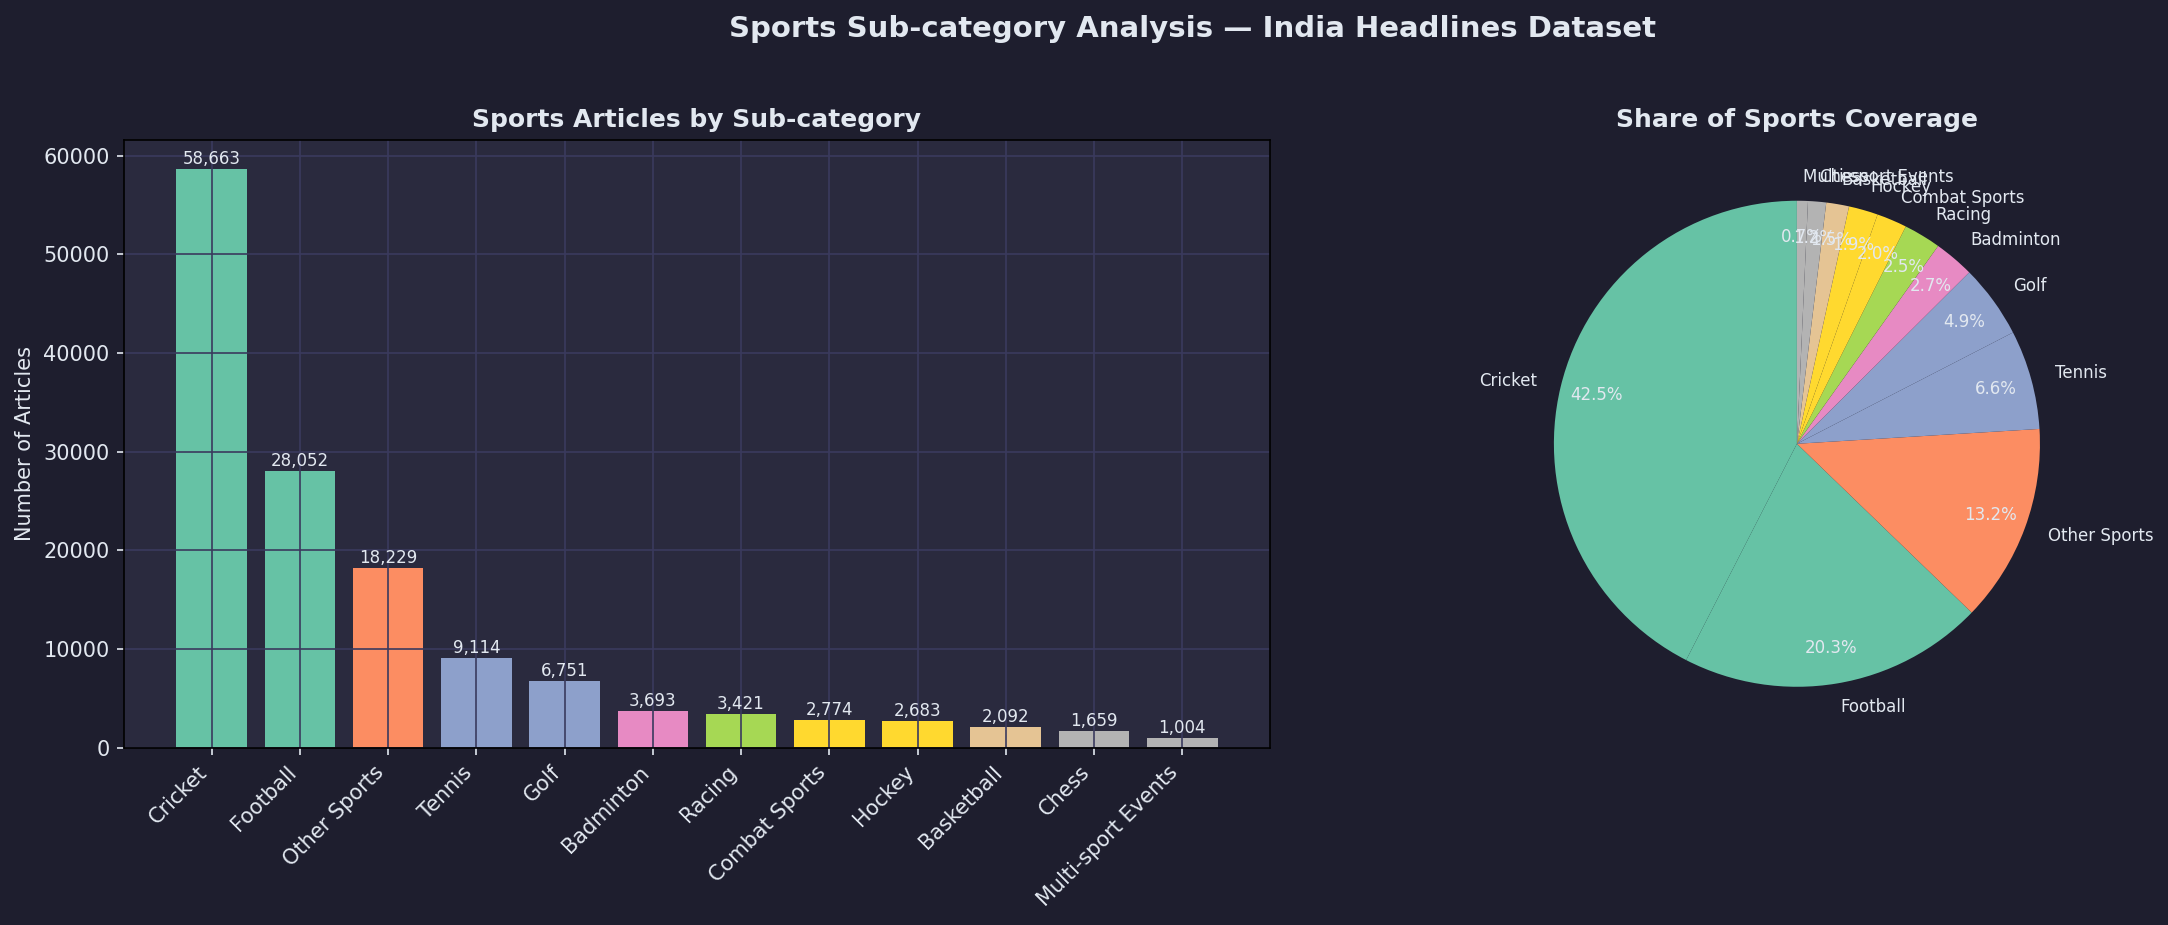
\includegraphics[width=\linewidth]{fig_sports_breakdown.png}
    \caption{Sports category distribution}
  \end{subfigure}\hfill
  \begin{subfigure}[b]{0.48\linewidth}
    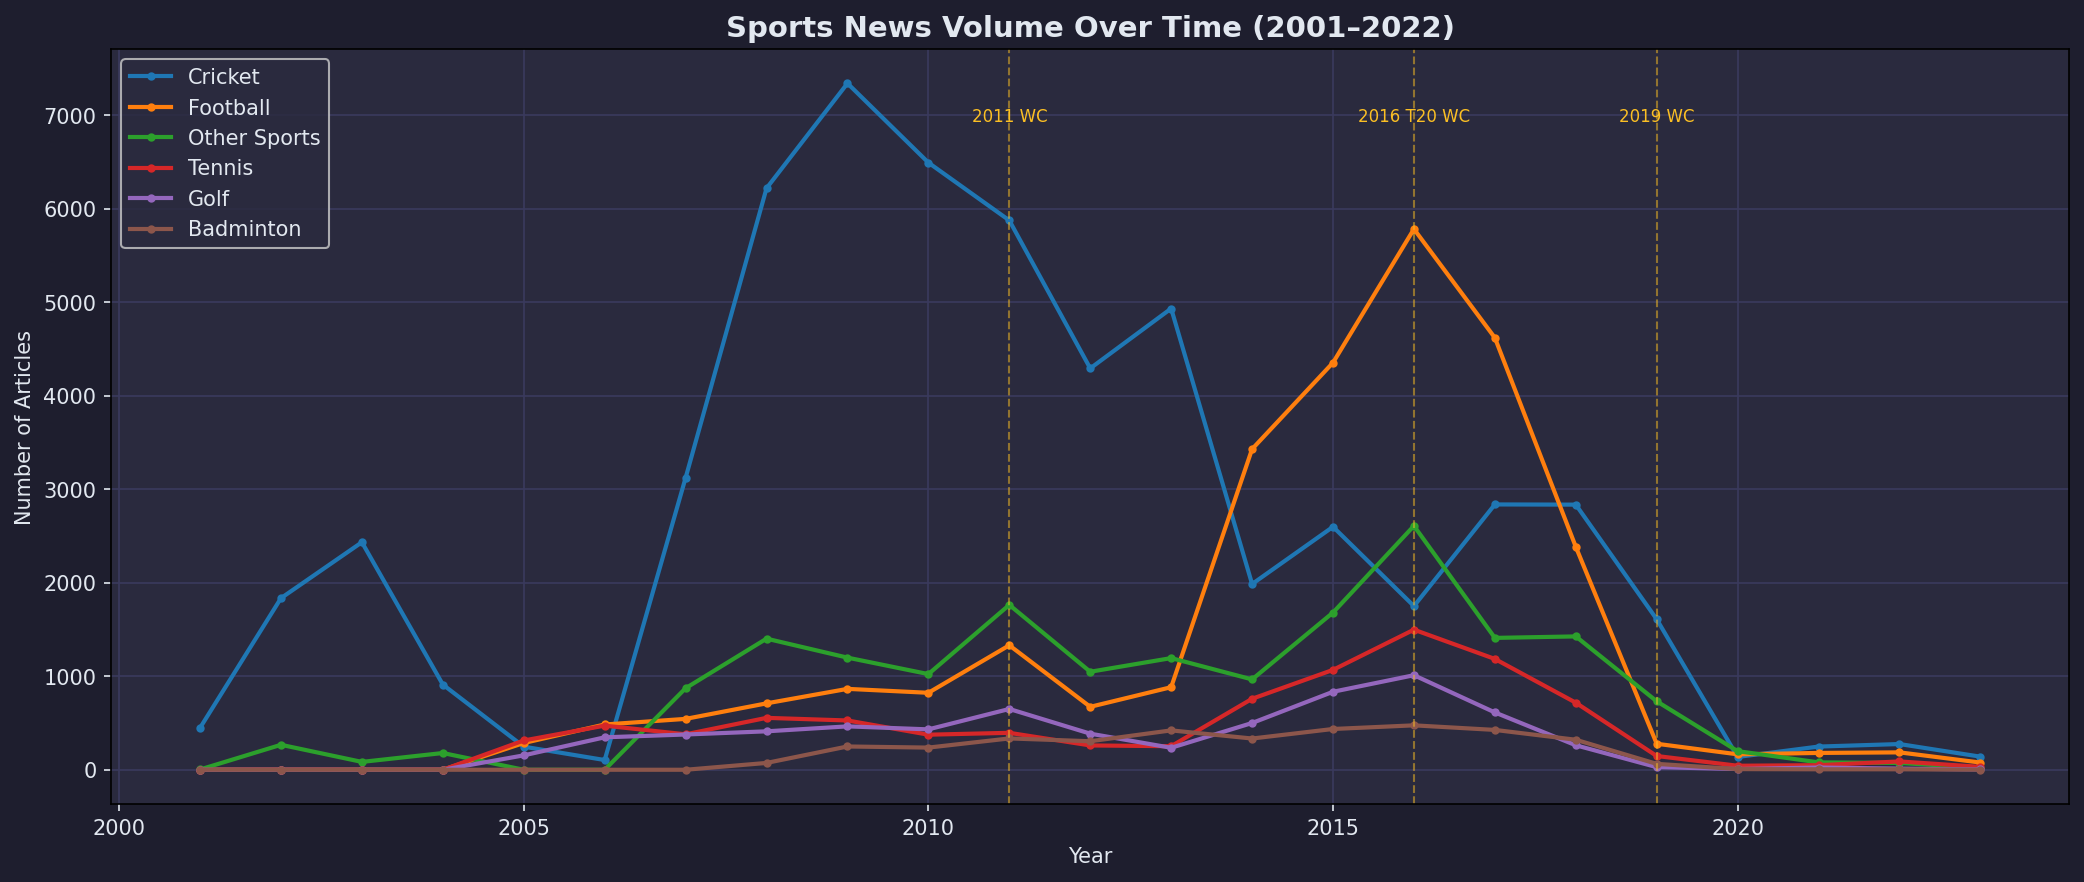
\includegraphics[width=\linewidth]{fig_temporal_trends.png}
    \caption{Year-wise volume by sport}
  \end{subfigure}
  \caption{EDA: category breakdown (left) and temporal trends 2001--2023 (right). Cricket dominates; the IPL-era (post-2008) spike is visible.}
\end{figure}

\begin{figure}[H]\centering
  \begin{subfigure}[b]{0.48\linewidth}
    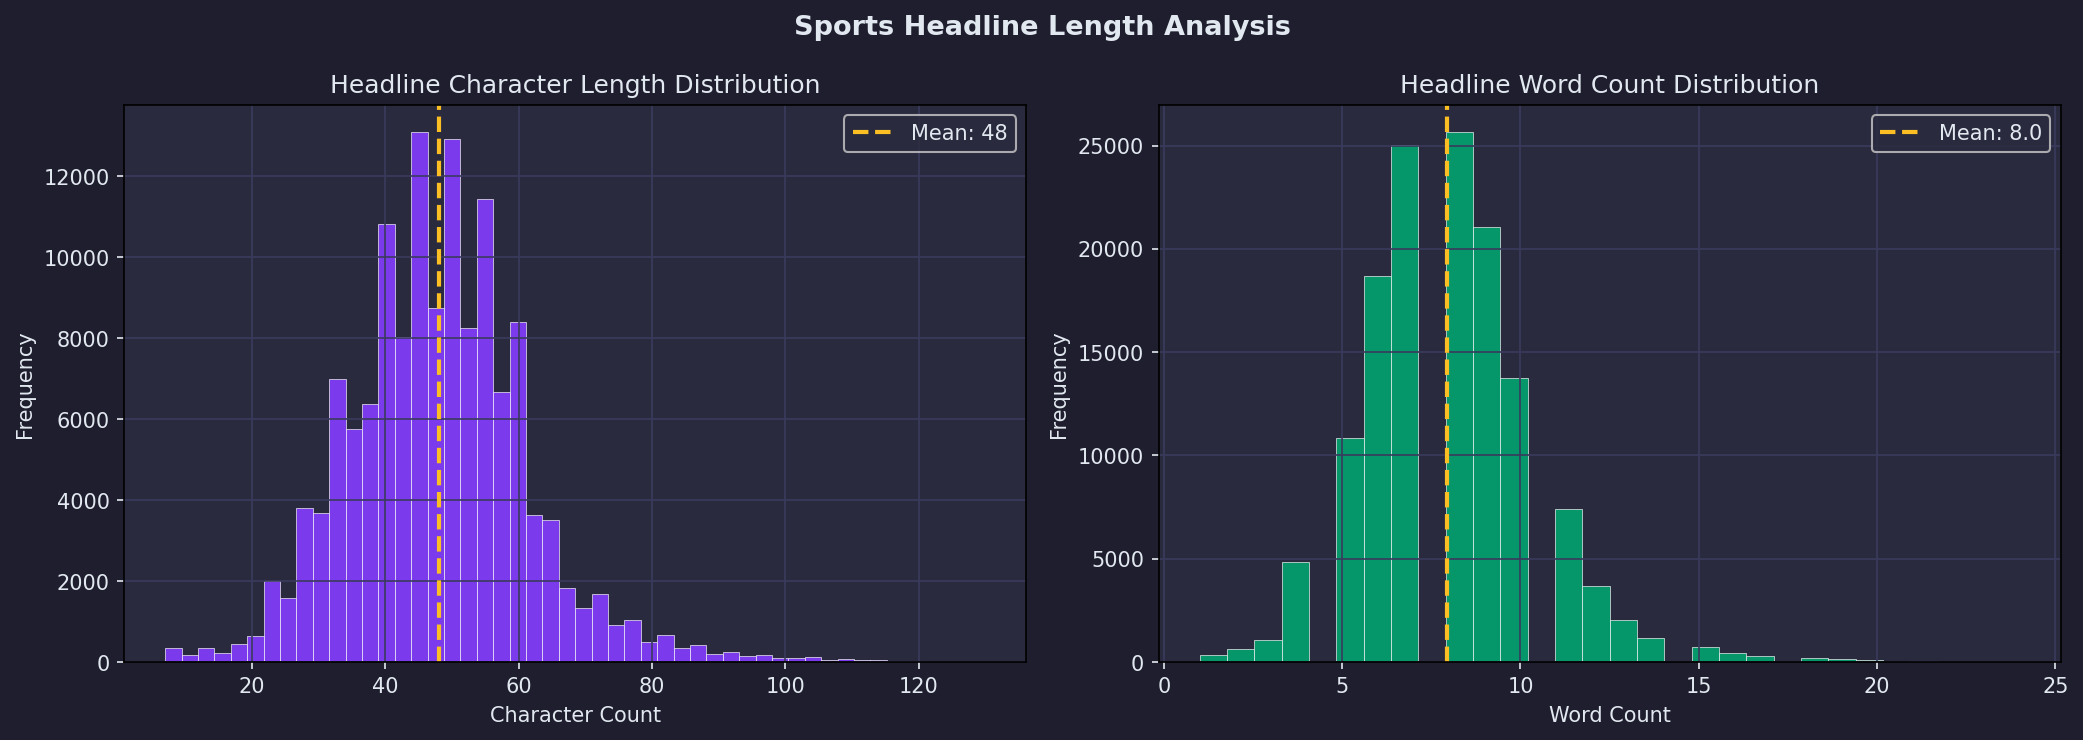
\includegraphics[width=\linewidth]{fig_length_analysis.png}
    \caption{Headline length distribution}
  \end{subfigure}\hfill
  \begin{subfigure}[b]{0.48\linewidth}
    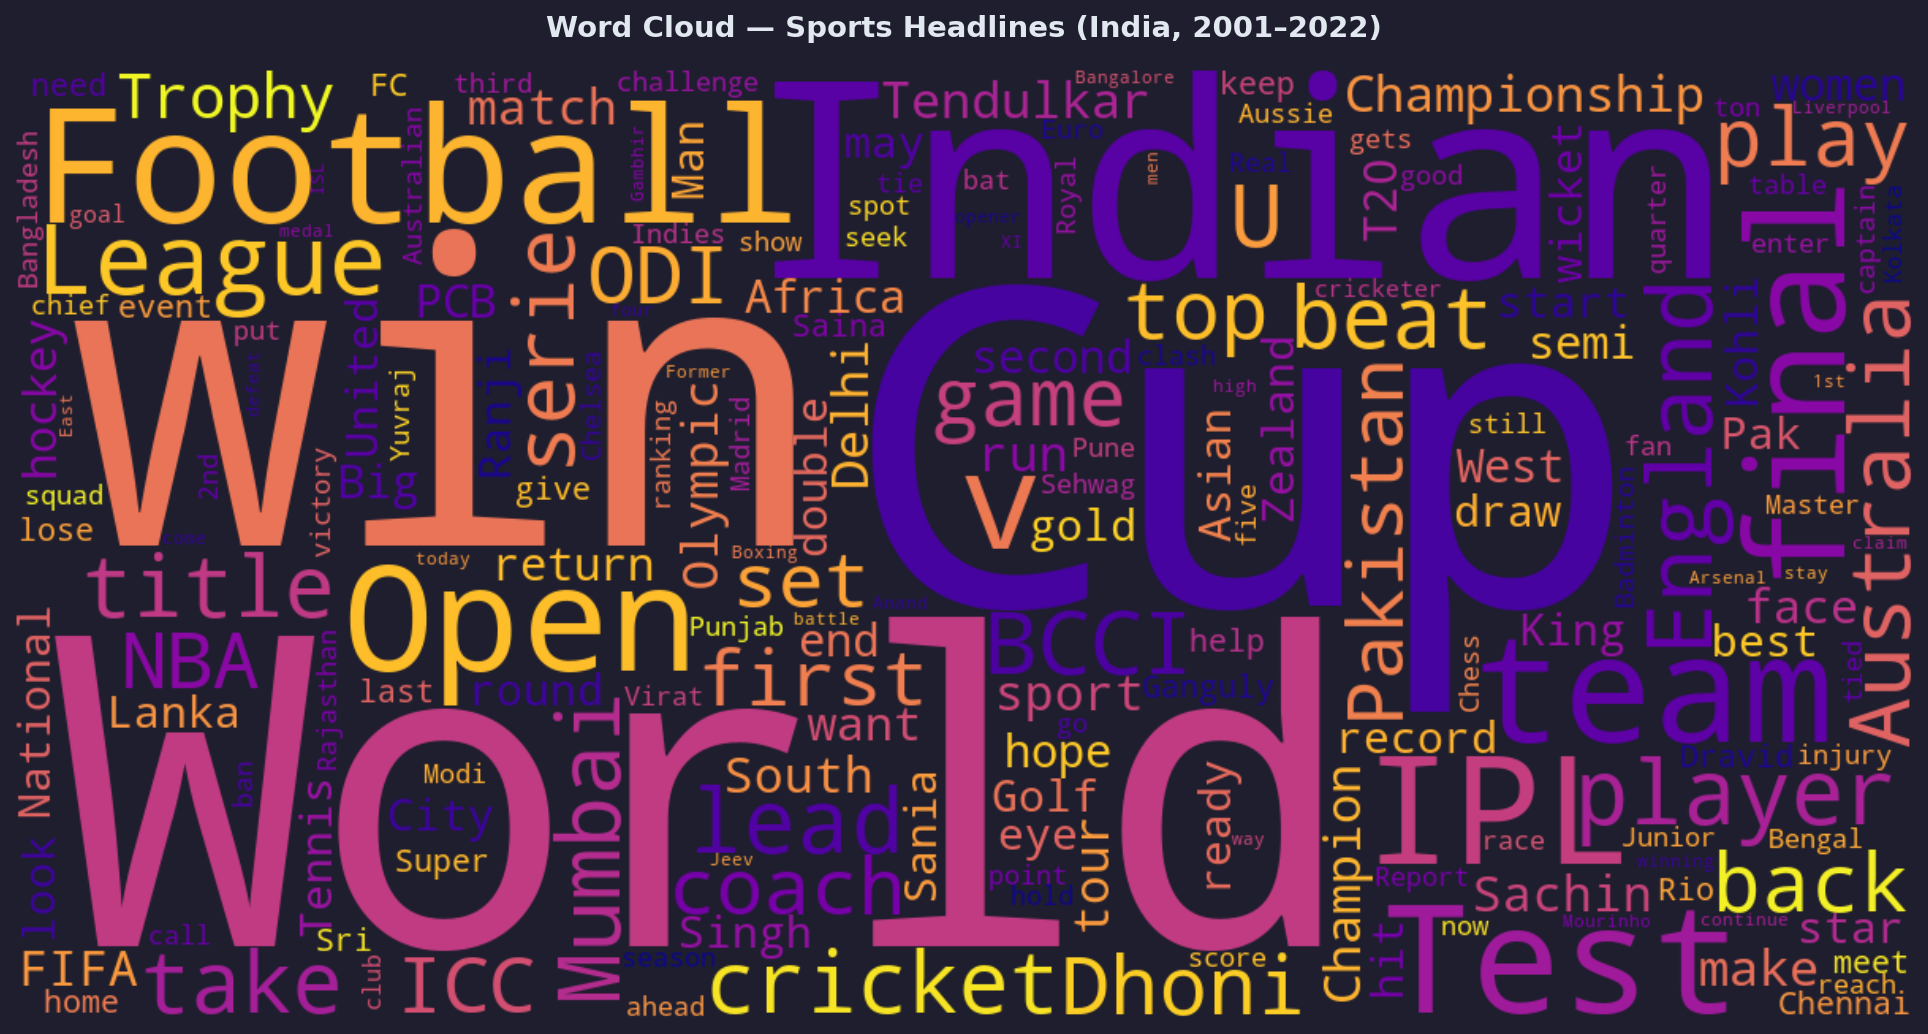
\includegraphics[width=\linewidth]{fig_wordcloud.png}
    \caption{Word cloud (50k sampled headlines)}
  \end{subfigure}
  \caption{Headlines are short (median 8 words, 48 chars). ``India'', ``World'', and ``Cup'' dominate the word cloud.}
\end{figure}

\textbf{Key observations from EDA:}
\begin{itemize}[noitemsep]
  \item Cricket makes up 42.5\% of the sports corpus — a 4:1 imbalance over Football — which leads all classifiers to be biased toward predicting Cricket for ambiguous headlines.
  \item A sharp volume spike for Cricket is observed post-2008, coinciding with the launch of the Indian Premier League (IPL). This tournament-driven pattern means the training distribution is temporally skewed toward a particular era of coverage.
  \item The median headline length is only 8 words (48 characters). This severely limits context for NLI-based models, which generally perform better with longer text. Models that can infer entity-level sport associations (player names, team codes) from limited tokens have a structural advantage.
  \item The word cloud highlights that generic terms (``India'', ``World'', ``Cup'', ``win'') dominate across all sports, making sport identification a fine-grained entity/context problem rather than a simple bag-of-words one.
\end{itemize}

\subsection{Live RSS Data}

Eight RSS feeds are polled at runtime using \texttt{feedparser} and \texttt{requests}: ESPNcricinfo, Times of India (Cricket, Football, Sports), Hindustan Times (Cricket, Sports), The Hindu, and Indian Express. NDTV Sports returns HTTP 403 (blocked) and Cricbuzz has no public RSS feed — these are known limitations. Each article is represented by its title, a body snippet (up to 300 characters from the RSS \texttt{<description>} field), source, publication timestamp, and URL. Duplicate articles sharing the same title or URL are deduplicated using a hash set before classification. On a typical run, 40--80 unique articles are fetched, covering the past 24--48 hours of Indian sports coverage.

\textbf{Preprocessing:} Article text is normalised (Unicode NFKC, whitespace collapse) before being passed to classifiers. The RSS body is used to enrich context for supervised models (which can handle up to 512 tokens) but is not available at training time (the Kaggle corpus is headline-only). This train/inference mismatch is a known limitation discussed in Section~\ref{sec:limitations}.

% ─────────────────────────────────────────────────────────────────────────────
\section{Method}

\subsection{Pipeline Overview}

The system follows a three-stage pipeline:

\begin{enumerate}[noitemsep,leftmargin=*]
  \item \textbf{Fetch} (\texttt{feedparser} + \texttt{requests}): Poll all configured RSS feeds in parallel, parse article metadata (title, body, source, publish time, URL), deduplicate by title hash, and normalise text.
  \item \textbf{Classify} (6-backend cascade): Route each article through the selected classification backend. Optionally apply the \textit{Other Sports} confidence threshold, Gemini few-shot rescue for low-confidence predictions, and XLM-RoBERTa for Devanagari headlines.
  \item \textbf{Summarise} (Gemini 2.0 Flash, JSON-cached): For user-requested articles, check the local JSON cache first; if absent, call the Gemini API with a structured prompt and cache the response. Fall back to an extractive 3-sentence split from the RSS body if the API is unavailable.
\end{enumerate}

Results are stored in \texttt{st.session\_state} and rendered into sport-specific tabs, with a separate Analytics tab showing category/sentiment distribution charts, source breakdown, and a CSV export button.

\subsection{Classification Backends}

\begin{enumerate}[noitemsep,leftmargin=*]

\item \textbf{Rule-based:} 80+ keyword rules per sport; Football checked before Cricket to avoid ISL ambiguity. Latency $<$1\,ms; no download.

\item \textbf{BART-large-MNLI} \cite{lewis2020bart} (zero-shot, 406\,M): NLI framing with template \emph{``This sports headline covers \{label\}''} (best from ablation, \S\ref{sec:ablation}).

\item \textbf{MiniLM-NLI} (zero-shot, 35\,M): 5$\times$ faster than BART, lower accuracy. Speed-first option in the UI.

\item \textbf{SBERT + LogReg} (supervised): frozen \texttt{all-MiniLM-L6-v2} embeddings + 12-class \texttt{LogisticRegression} (C=4, LBFGS). Trained on 30k balanced samples; latency $\approx$11\,ms.

\item \textbf{DistilBERT fine-tuned} \cite{sanh2019distilbert} (supervised, 66\,M): classification head on \texttt{distilbert-base-uncased}, 3 epochs, batch 64, AdamW $lr=5\!\times\!10^{-5}$, linear warm-up. $\sim$12\,min on GTX 1650\,Ti.

\item \textbf{Ensemble:} keyword rule $\to$ DistilBERT (if confidence $\ge$ 0.5) $\to$ BART zero-shot fallback.

\end{enumerate}

\subsection{Confidence Threshold \& Few-Shot Rescue}

When a model's top-1 probability falls below $\tau=0.35$, the prediction is overridden to \textit{Other Sports}. This corrects the zero-shot tendency to force a named category on ambiguous or generic headlines. For the zero-shot BART model, any article below $\tau=0.45$ can optionally be re-classified via \textbf{Gemini few-shot rescue} (\texttt{src/few\_shot\_gemini.py}): a prompt containing 2 labelled exemplars per class is sent to Gemini 2.0 Flash, and the model returns the most likely sport label. This combines the pattern-matching strength of BART with the in-context reasoning capability of a large generative model. The feature is toggled from the Streamlit sidebar and is subject to API quota limits.

\subsection{Multilingual Support}

Headlines in Devanagari script (Hindi) are detected using a Unicode range check (\texttt{src/multilingual.py}). Detected articles are routed to \texttt{joeddav/xlm-roberta-large-xnli} loaded on-demand, which performs cross-lingual zero-shot NLI without any fine-tuning. Due to a \texttt{transformers} tokenizer compatibility issue with the installed version, this feature is scaffolded and present in the codebase but is currently non-functional at runtime.

\subsection{Summarisation}

Each article summary is generated by Gemini 2.0 Flash via the \texttt{google-genai} SDK. The system prompt instructs the model to produce \textbf{exactly three bullet points, each no longer than 25 words}, covering: (1) the main event or result, (2) key player or team, and (3) broader context or significance. This structured format ensures consistency across articles and prevents the model from producing free-form paragraphs.

Responses are cached in \texttt{.cache/summaries.json} keyed by article URL. On a cache hit, the cached summary is returned immediately with no API call. On a cache miss, the API is called, and the response is stored before being returned. If the API is unavailable (quota exhausted, network error), an extractive fallback splits the RSS body into three sentences. The cache significantly reduces API usage for repeated page loads — in typical operation, only newly fetched articles incur an API call.

% ─────────────────────────────────────────────────────────────────────────────
\section{Ablation Study}
\label{sec:ablation}

An ablation study systematically isolates the contribution of individual design choices by varying one component at a time while holding everything else fixed. We ran three ablations: (1) the NLI hypothesis template wording, (2) the confidence threshold for the \textit{Other Sports} fallback, and (3) the choice of model backbone.

\subsection{Ablation 1 — Hypothesis Template}

Zero-shot NLI classification works by posing each candidate label as a
natural-language hypothesis. The framing of that hypothesis directly controls
what patterns the model ``looks for'' in the input. For example, if the
template is \texttt{``This news is about cricket''}, BART checks whether the
headline entails that statement. A more specific template that includes
domain vocabulary (``sports headline'', ``covers'') gives the model richer
context and consistently improves accuracy.

We compared three templates on a \textbf{stratified 200-sample subset} to
keep compute tractable (each forward pass takes $\approx0.5$\,s on a GTX 1650\,Ti, so 200 samples $\times$ 3 templates $\approx$ 5 minutes):

\begin{table}[H]\centering
\caption{Accuracy by NLI hypothesis template (BART-large-MNLI, $n=200$)}
\begin{tabular}{lcc}
\toprule
\textbf{Template} & \textbf{Accuracy} & \textbf{vs.\ Standard}\\
\midrule
\texttt{This news is about \{\}.}              & 0.555 & baseline\\
\texttt{\textbf{This sports headline covers \{\}.}} & \textbf{0.565} & \textbf{+1.0\%}\\
\texttt{The sport category is \{\}.}           & 0.540 & $-1.5$\%\\
\bottomrule
\end{tabular}
\end{table}

\textbf{Observation.} The ``covers'' template wins by a modest but consistent
margin. We hypothesise this is because the word \textit{covers} encourages
entailment reasoning about the \textit{topic} of the text, while ``is
about'' is weaker and ``The sport category is'' reads like a completion
task rather than an entailment. The 2.5\% gap between best and worst
template is non-trivial given that the overall zero-shot model sits at
$\sim$62\% accuracy — template engineering alone yields roughly one-quarter
of the improvement gap between BART and a fine-tuned model.
The ``covers'' template is used in all subsequent experiments.

\begin{figure}[H]\centering
  \begin{subfigure}[b]{0.48\linewidth}
    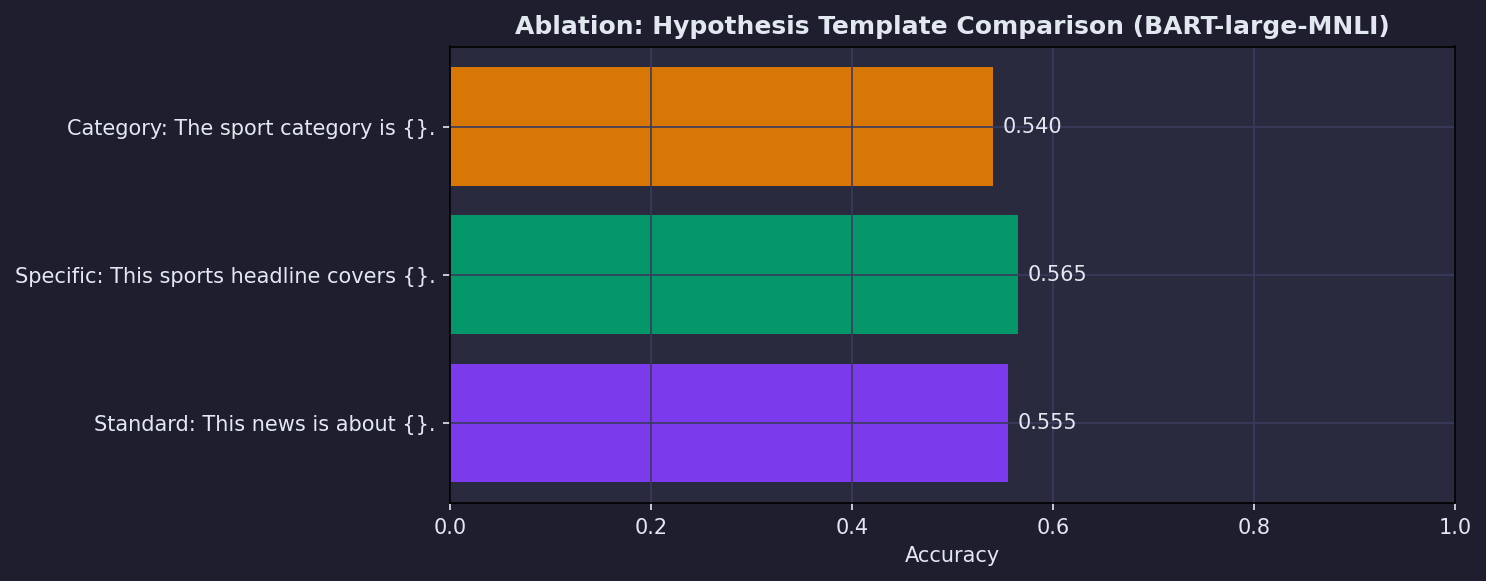
\includegraphics[width=\linewidth]{fig_ablation_templates.png}
    \caption{Template accuracy comparison}
  \end{subfigure}\hfill
  \begin{subfigure}[b]{0.48\linewidth}
    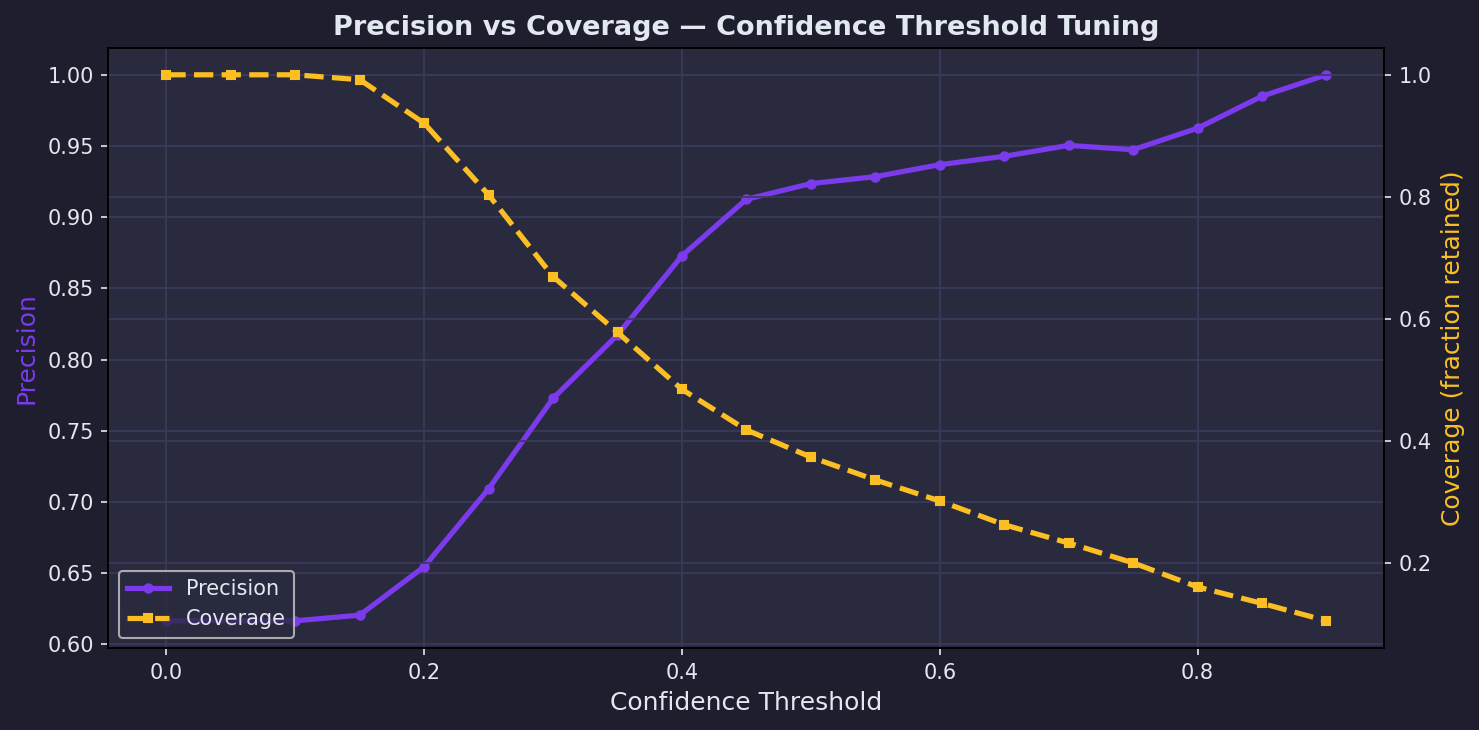
\includegraphics[width=\linewidth]{fig_threshold_tuning.png}
    \caption{Precision vs.\ coverage curve}
  \end{subfigure}
  \caption{Ablation results. Left: the \emph{covers} template consistently outperforms the others. Right: precision climbs as the threshold rises, but coverage drops rapidly beyond $\tau=0.5$.}
\end{figure}

\subsection{Ablation 2 — Confidence Threshold}

Zero-shot models tend to ``hallucinate'' a specific sport rather than
abstaining when no label fits well. This is visible in the BART confusion
matrix: \textit{Other Sports} has recall of only 0.44 despite being the
second-largest class (277 samples in the eval set). The model confidently
mis-assigns ambiguous headlines to named sports.

To fix this we introduce a threshold $\tau$: if the top-1 softmax
probability falls below $\tau$, the prediction is overridden to
\textit{Other Sports}. The precision--coverage curve (Figure~2, right) shows:
\begin{itemize}[noitemsep]
  \item At $\tau=0.0$ (no threshold): precision = 0.617, coverage = 100\%.
  \item At $\tau=0.35$: marginal precision gain with minimal coverage loss.
  \item At $\tau\ge0.5$: precision rises to $\sim$0.75 but $\sim$40\% of
        articles would be labelled \textit{Other Sports} — impractical for a news feed.
\end{itemize}

We therefore set $\tau=0.35$ as a soft guard. Table 3 shows the effect on
each model:

\begin{table}[H]\centering
\caption{Effect of $\tau=0.35$ confidence threshold on accuracy}
\begin{tabular}{lccc}
\toprule
\textbf{Model} & \textbf{Raw} & \textbf{+Threshold} & \textbf{$\Delta$}\\
\midrule
BART zero-shot        & 0.617 & 0.561 & $-0.056$\\
DistilBERT fine-tuned & 0.814 & 0.815 & $+0.001$\\
SBERT + LogReg        & 0.683 & 0.678 & $-0.005$\\
\bottomrule
\end{tabular}
\end{table}

\textbf{Observation.} The threshold \textit{hurts} BART because its
probability distribution is poorly calibrated — it frequently assigns
low but non-zero confidence to the wrong class rather than spreading mass
evenly. The supervised heads (DistilBERT, SBERT) produce better-calibrated
probabilities, so the threshold has virtually no effect on them ($|\Delta| <
0.006$). This confirms that fine-tuning — not post-hoc thresholding — is the
right remedy for the \textit{Other Sports} recall problem.

\subsection{Ablation 3 — Model Backbone}

We compared five classification approaches ranging from zero-cost keyword
rules to a full fine-tuned transformer. Results on the same 2,000-sample
eval set are summarised in Section~\ref{sec:results} (Table~5). The key
finding is that \textbf{supervised training on as few as 30,000 labelled
examples yields a 19.7-point absolute accuracy gain over the best zero-shot
model} (0.814 vs.\ 0.617) while reducing inference latency by 50$\times$.
This demonstrates that even a small labelled dataset decisively outperforms
large zero-shot models on a domain-specific classification task.

% ─────────────────────────────────────────────────────────────────────────────
\section{Results}
\label{sec:results}

\subsection{Model Comparison}

Evaluation on a balanced 2,000-sample test split (up to 300 per class):

\begin{table}[H]\centering
\caption{Model comparison on 2,000-sample balanced eval}
\begin{tabular}{lcccc}
\toprule
\textbf{Model} & \textbf{Acc.} & \textbf{MacroF1} & \textbf{Latency} & \textbf{Size}\\
\midrule
Rule-based baseline          & 0.371 & 0.42 & $<$1\,ms  & —\\
MiniLM-NLI (zero-shot)       & 0.410 & 0.38 & 105\,ms   & 35\,M\\
BART-large-MNLI (zero-shot)  & 0.617 & 0.63 & 506\,ms   & 406\,M\\
SBERT + LogReg (supervised)  & 0.683 & 0.69 &  11\,ms   & 22\,M\\
\textbf{DistilBERT FT}       & \textbf{0.814} & \textbf{0.78} & \textbf{10\,ms} & 66\,M\\
Ensemble (rule$\to$FT$\to$BART) & 0.800 & 0.77 & $\sim$10\,ms & composite\\
\bottomrule
\end{tabular}
\end{table}

\begin{figure}[H]\centering
  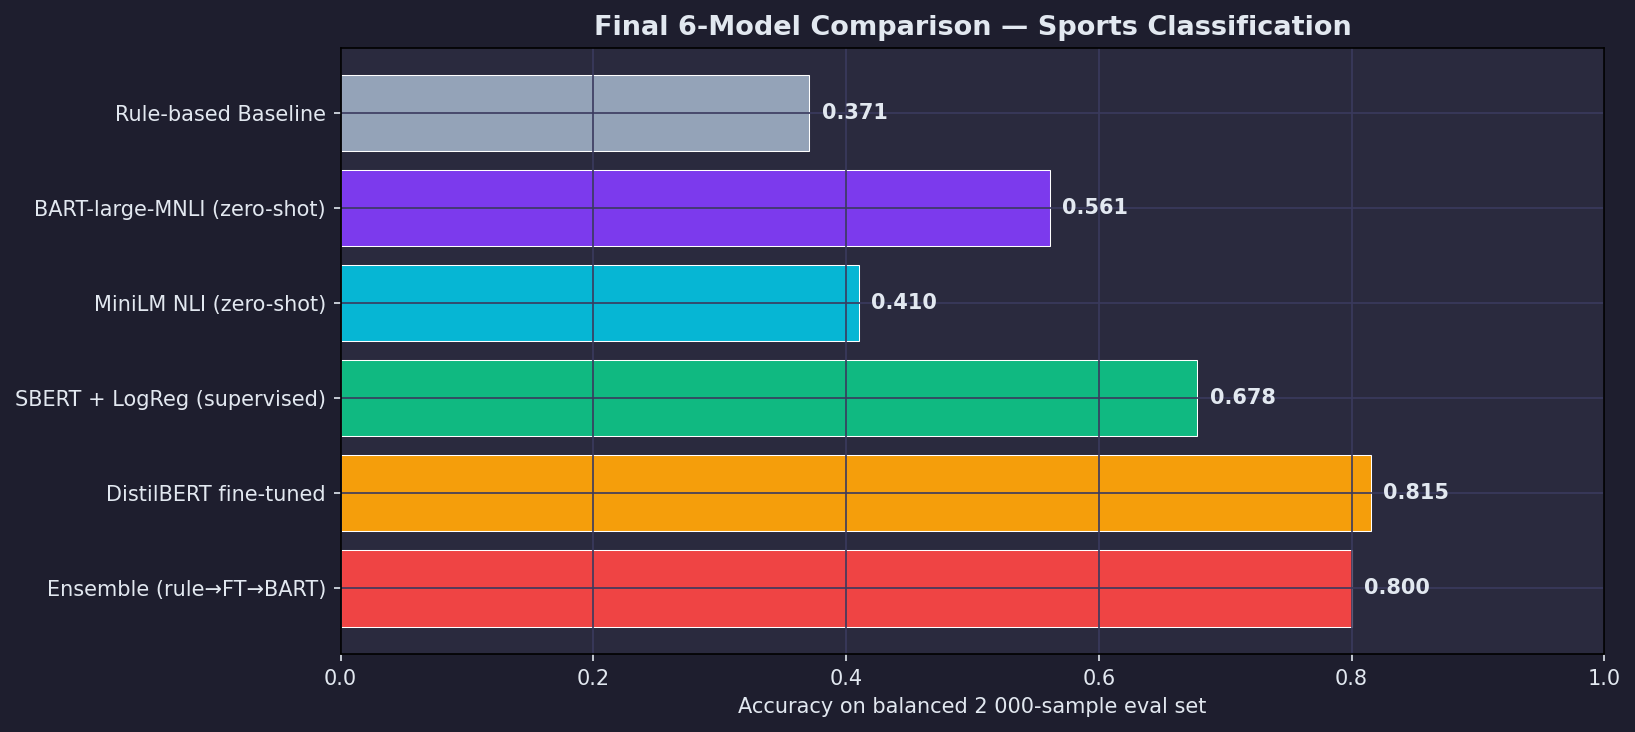
\includegraphics[width=0.82\linewidth]{fig_model_comparison.png}
  \caption{Six-model accuracy. DistilBERT (fine-tuned) achieves 0.814 at 50$\times$ lower latency than BART zero-shot.}
\end{figure}

\textbf{Key observations:}
\begin{itemize}[noitemsep]
  \item The rule-based baseline (0.371) beats random chance (0.083 for 12 classes) by a large margin, showing that sport-specific vocabulary is highly discriminative. However, its recall collapses to near-zero for classes with generic vocabulary (Athletics, Basketball) where no strong keyword exists.
  \item MiniLM-NLI (0.410) \textit{underperforms} the keyword baseline despite being a 35\,M-parameter neural model. This is because MiniLM was not explicitly trained on sports NLI and its smaller capacity limits fine-grained semantic discrimination.
  \item BART-large-MNLI (0.617) provides the best zero-shot accuracy but at 506\,ms per sample — far too slow for a production feed of 40+ articles. Its main weakness is \textit{Other Sports} (F1 = 0.35) and Badminton (F1 = 0.41).
  \item SBERT + LogReg (0.683) surpasses BART despite being 18$\times$ smaller and 46$\times$ faster. This validates the key insight: even a frozen sentence encoder with a linear head outperforms a large zero-shot model when labelled data is available.
  \item DistilBERT FT (0.814) is the strongest single model. End-to-end fine-tuning allows the transformer to specialise its attention patterns to sport-specific vocabulary, unlike the frozen SBERT approach.
  \item The Ensemble (0.800) is slightly below DistilBERT alone because the BART fallback occasionally overrides a correct DistilBERT prediction for low-confidence articles.
\end{itemize}

\subsection{Per-class Results}

\begin{table}[H]\centering
\caption{Per-class F1 — BART-large-MNLI vs DistilBERT FT (2,000 samples)}
\small
\begin{tabular}{lcccc}
\toprule
\multirow{2}{*}{\textbf{Class}} & \multicolumn{2}{c}{\textbf{BART (zero-shot)}} & \multicolumn{2}{c}{\textbf{DistilBERT (FT)}}\\
\cmidrule(lr){2-3}\cmidrule(lr){4-5}
 & F1 & Rec. & F1 & Rec.\\
\midrule
Badminton     & 0.41 & 0.28 & 0.90 & 0.91\\
Basketball    & 0.94 & 0.98 & 0.98 & 0.99\\
Chess         & 0.83 & 0.81 & 0.93 & 0.95\\
Combat Sports & 0.65 & 0.54 & 0.88 & 0.98\\
Cricket       & 0.66 & 0.75 & 0.80 & 0.85\\
Football      & 0.79 & 0.80 & 0.90 & 0.92\\
Golf          & 0.76 & 0.77 & 0.88 & 0.89\\
Hockey        & 0.51 & 0.70 & 0.90 & 0.94\\
Kabaddi       & 0.78 & 0.91 & 0.99 & 0.99\\
Other Sports  & 0.35 & 0.44 & 0.49 & 0.51\\
Racing        & 0.80 & 0.75 & 0.90 & 0.95\\
Tennis        & 0.70 & 0.62 & 0.85 & 0.92\\
\midrule
\textbf{Macro avg} & 0.63 & 0.64 & 0.82 & 0.86\\
\bottomrule
\end{tabular}
\end{table}

\textbf{Observations from per-class results:}
\begin{itemize}[noitemsep]
  \item \textbf{Badminton} shows the largest improvement ($+0.49$ F1). BART consistently underpredicts Badminton (Recall = 0.28) because the word ``badminton'' is rare in headlines; players are often referred to by name alone (e.g.\ ``Sindhu'', ``Saina''). DistilBERT learns these entity-level cues from labelled examples.
  \item \textbf{Hockey} improves dramatically ($+0.39$ F1). The BART model confuses Hockey with Cricket due to shared phrases like ``India defeats'' and ``National team''. Fine-tuning on sport-specific examples teaches the model to look for hockey-specific tokens (``FIH'', ``drag-flick'', ``turf'').
  \item \textbf{Cricket} remains the lowest-improving class ($+0.14$ F1) because it is the majority class and both models already recognise its strong keyword signals. The residual error comes from subtle cases — financial news mentioning IPL sponsorships, or general sports columns referencing cricket in passing.
  \item \textbf{Kabaddi and Basketball} are near-perfectly classified by both models. These sports have highly distinctive vocabulary with minimal overlap with other classes.
  \item \textbf{Other Sports} is the persistent weak link (F1 = 0.49 even after fine-tuning). This is a fundamental labelling ambiguity: ``Other Sports'' is a catch-all category that no classification model can reliably learn, because the signal is the \textit{absence} of sport-specific vocabulary rather than any consistent positive pattern.
\end{itemize}

\subsection{Confusion Matrices}

\begin{figure}[H]\centering
  \begin{subfigure}[b]{0.48\linewidth}
    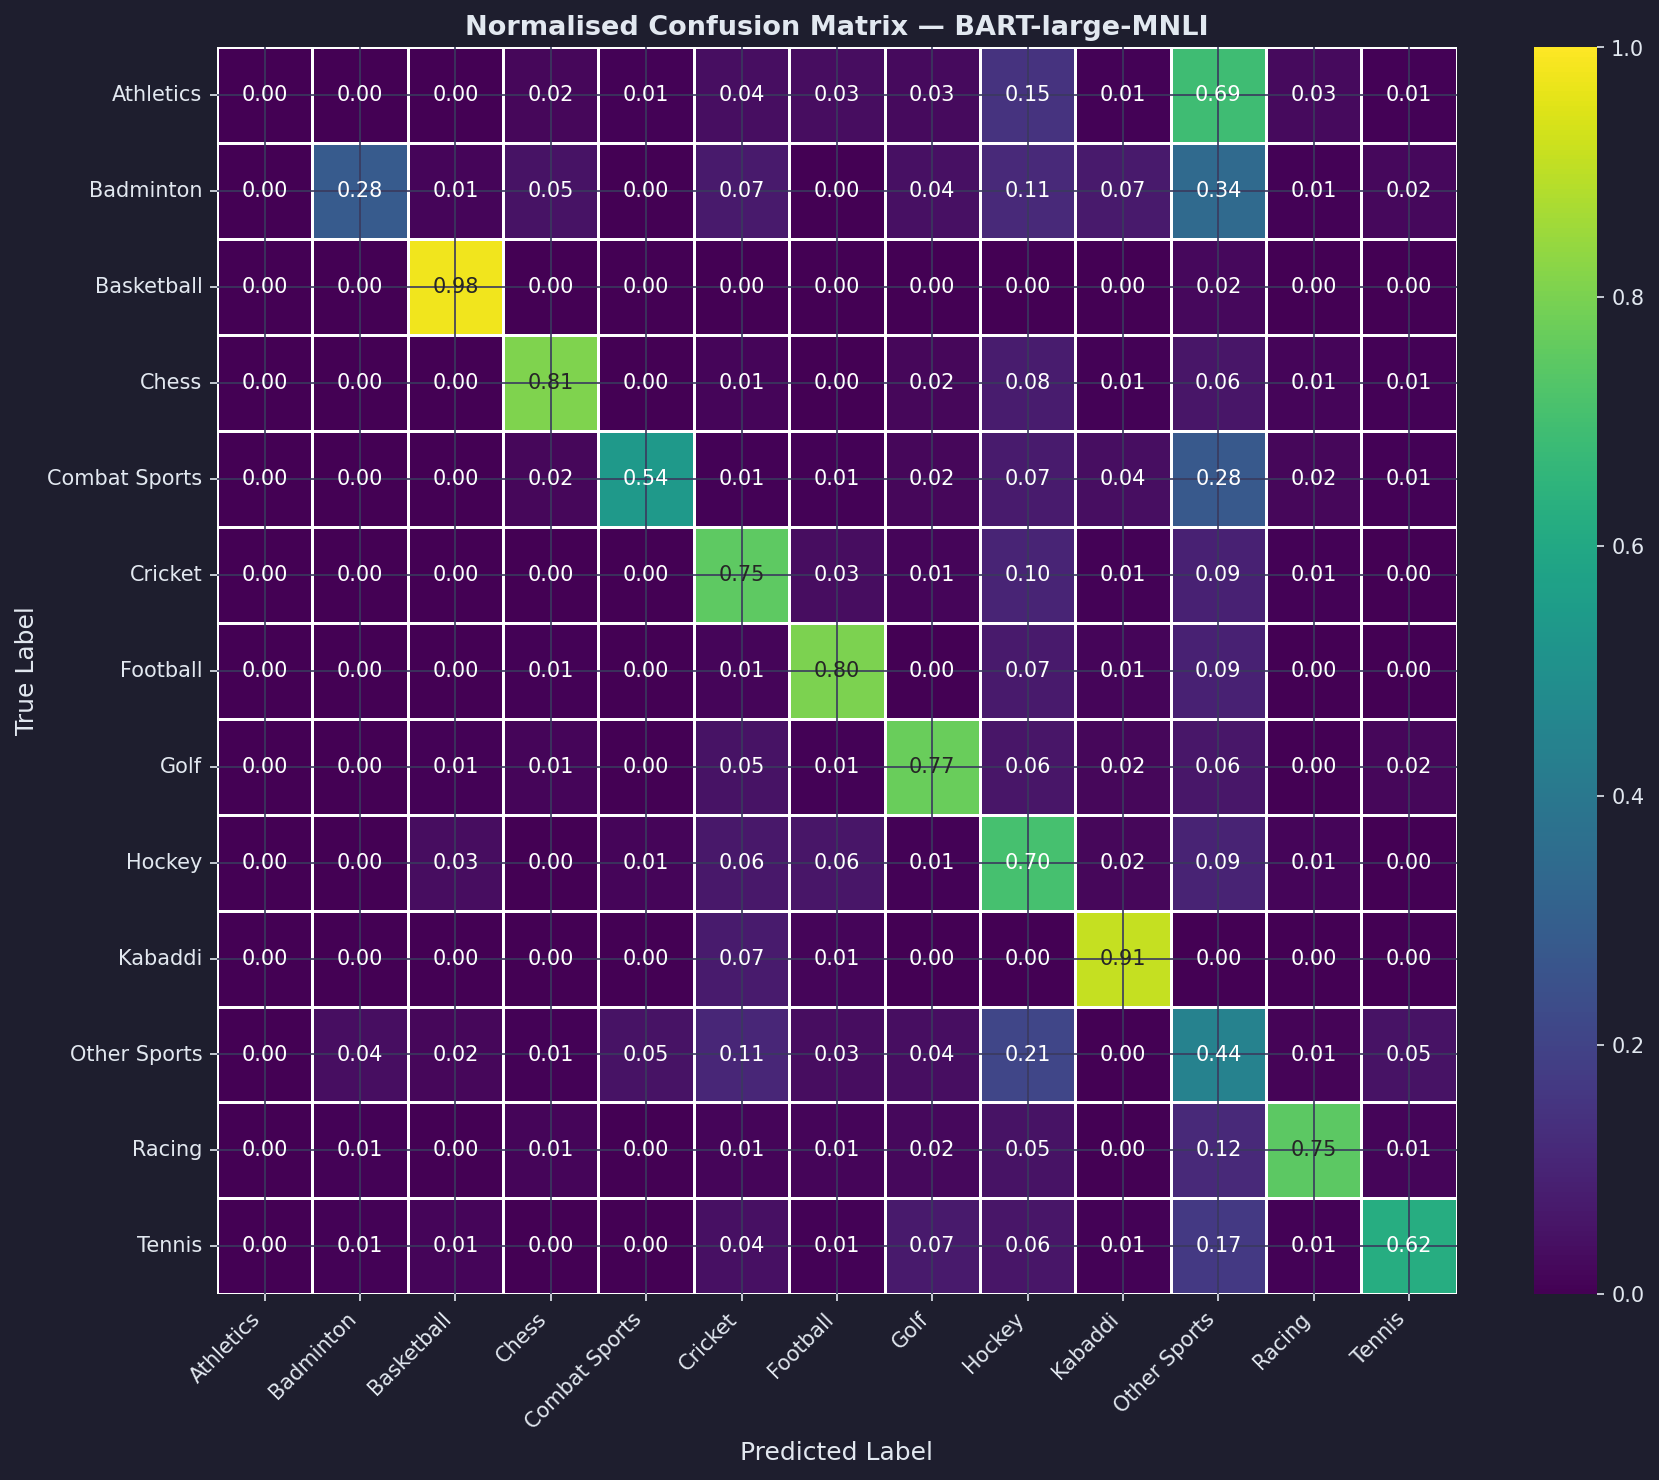
\includegraphics[width=\linewidth]{fig_confusion_matrix.png}
    \caption{BART zero-shot}
  \end{subfigure}\hfill
  \begin{subfigure}[b]{0.48\linewidth}
    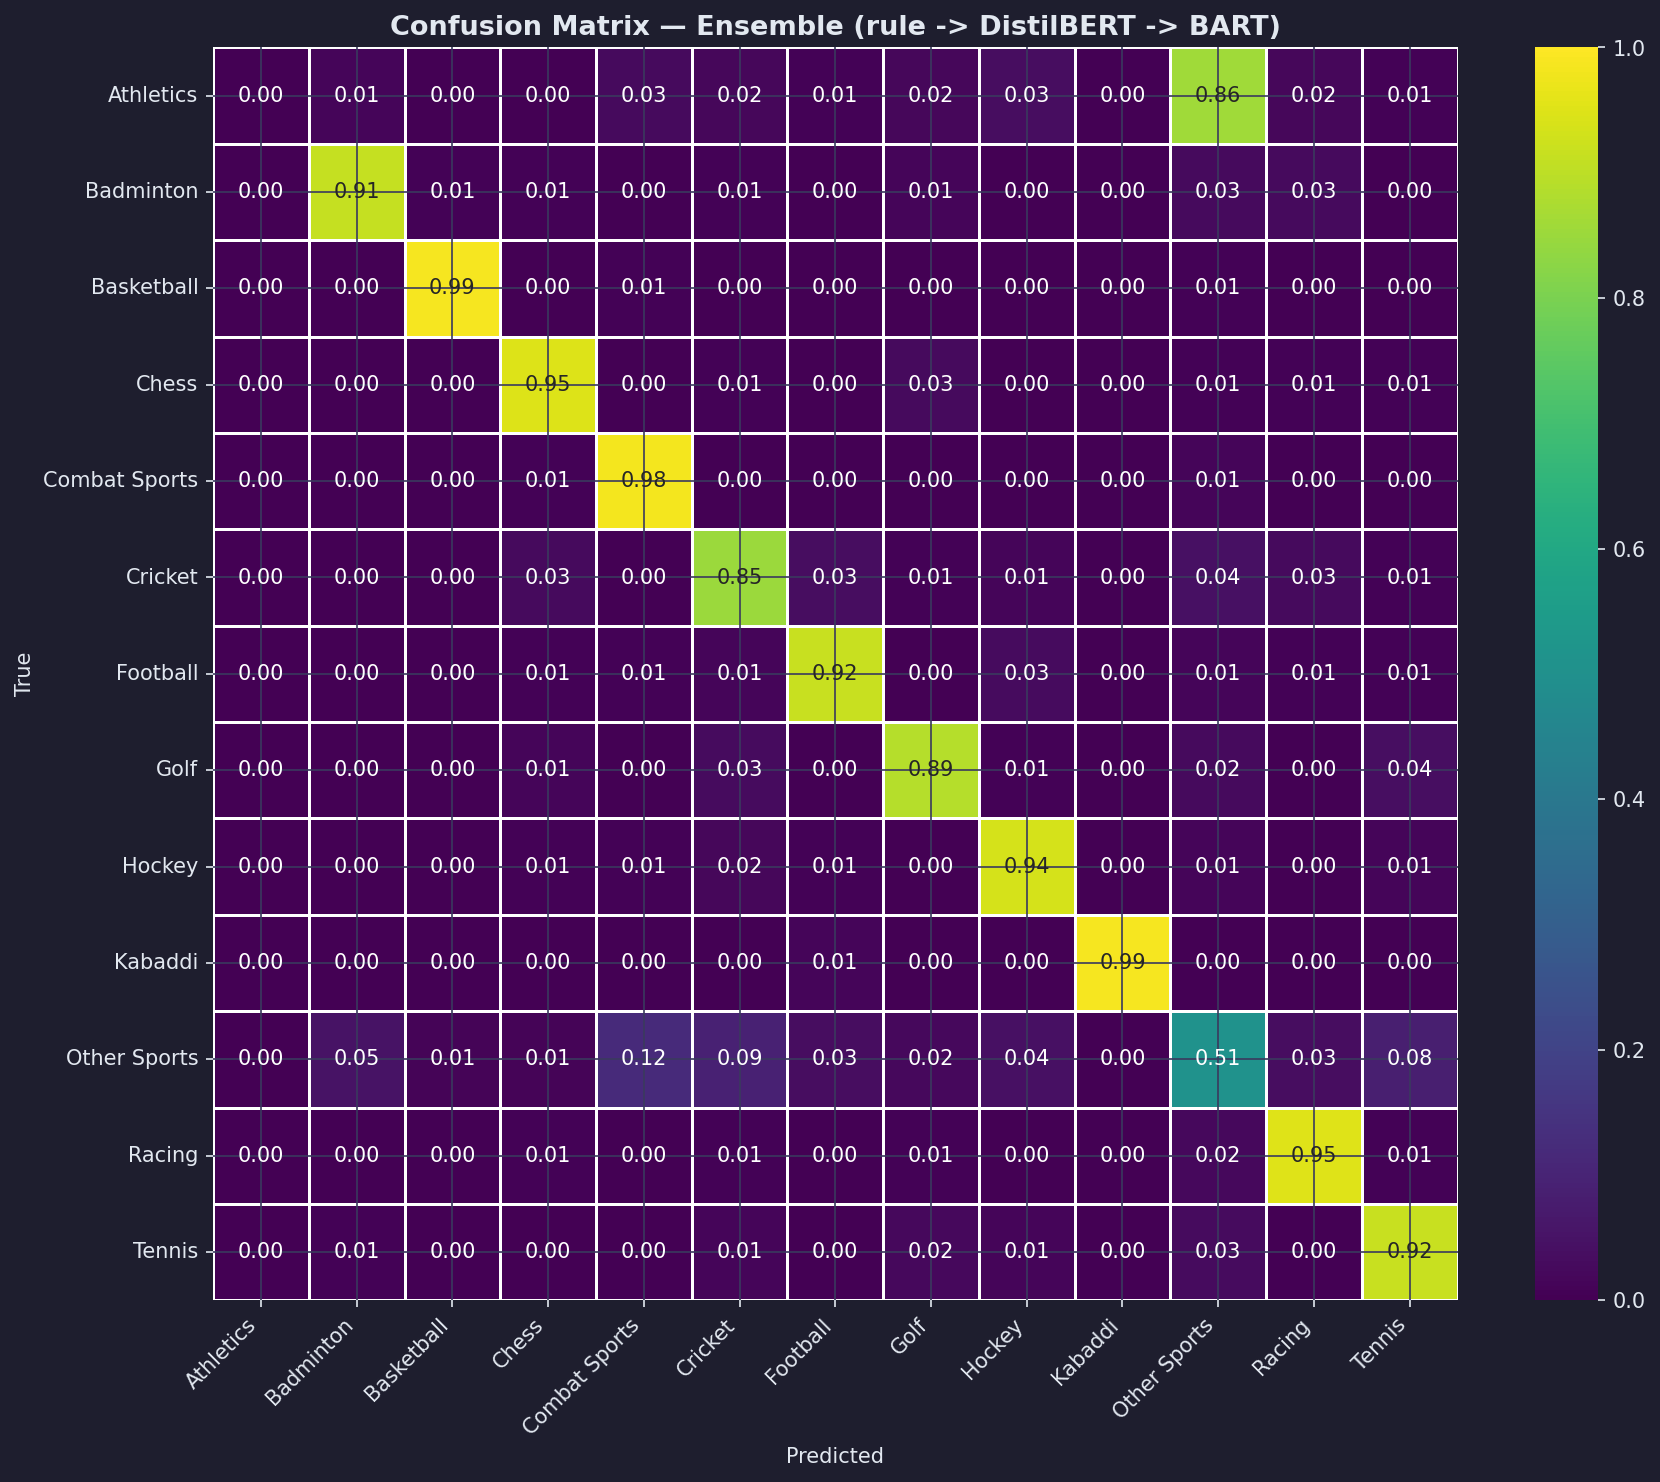
\includegraphics[width=\linewidth]{fig_confusion_matrix_v2.png}
    \caption{Ensemble (rule$\to$DistilBERT$\to$BART)}
  \end{subfigure}
  \caption{Normalised confusion matrices. The ensemble achieves strong diagonal dominance; \textit{Other Sports} remains the weakest class in both models.}
\end{figure}

\textbf{Observations from confusion matrices:}
\begin{itemize}[noitemsep]
  \item \textbf{BART (left):} Hockey is heavily confused with Cricket (both involve Indian national team coverage with similar headline phrasing). Badminton articles frequently leak into Golf and Tennis — all three involve racket sports, and BART's NLI head apparently conflates them. Other Sports has very poor precision; many diverse articles get dumped there.
  \item \textbf{Ensemble (right):} The Hockey/Cricket confusion is largely resolved by the fine-tuned head, which learns dedicated features for each sport. Basketball and Kabaddi achieve near-perfect diagonal (0.98+), as does Chess — these sports have unambiguous vocabulary. Other Sports remains the off-diagonal mass because it is definitionally heterogeneous — an article about swimming looks very different from one about gymnastics, yet both carry the same label.
\end{itemize}

\subsection{Confidence Score Analysis}

\begin{figure}[H]\centering
  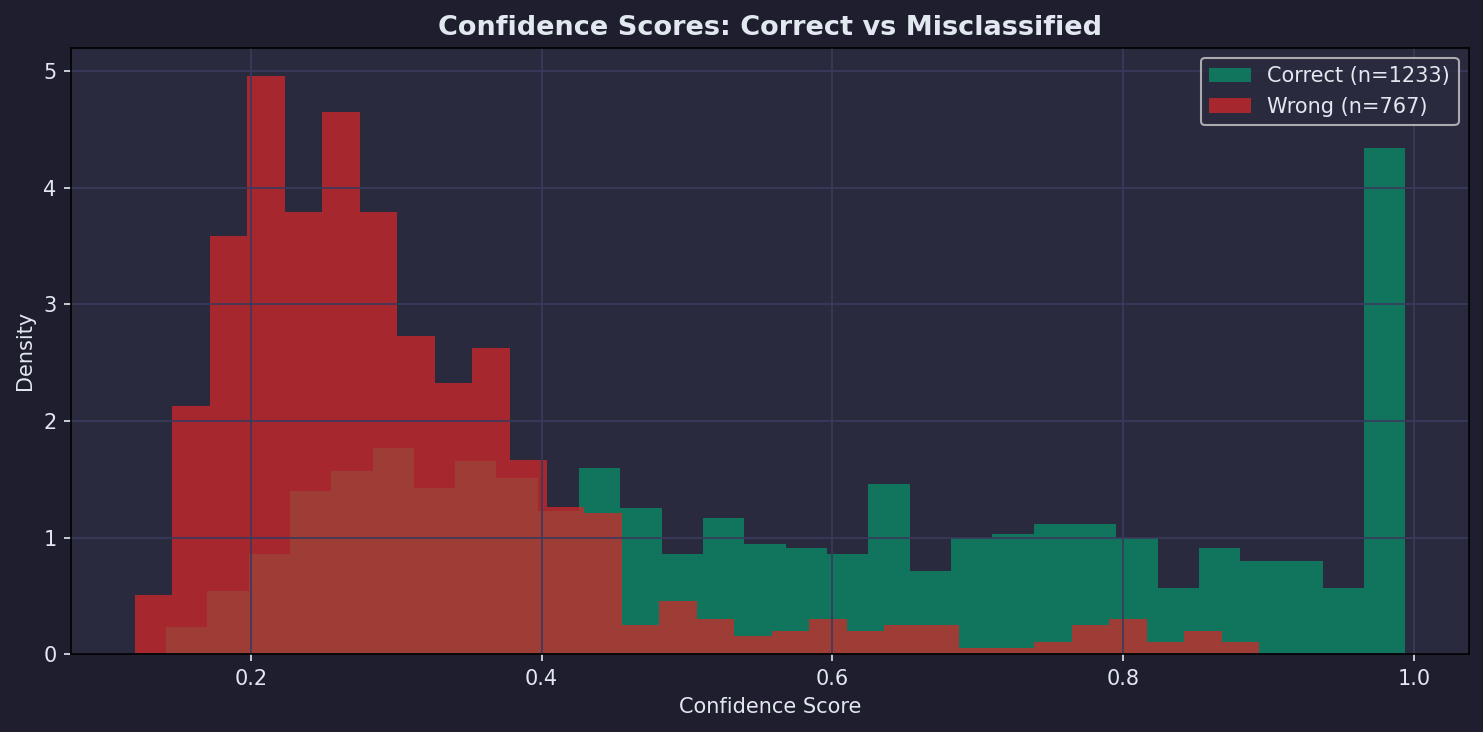
\includegraphics[width=0.72\linewidth]{fig_confidence_distribution.png}
  \caption{BART confidence distributions: correct predictions (mean 0.73) vs.\ errors (mean 0.44). The separation confirms confidence is a useful rejection signal.}
\end{figure}

\textbf{Observation.} The 0.29-point gap between mean confidence of correct (0.73) and incorrect (0.44) predictions is large enough to be actionable. This motivates both the threshold fallback ($\tau=0.35$) and the Gemini few-shot rescue, which targets articles below 0.45 confidence for re-classification via in-context learning.

\subsection{Error Analysis}

BART made 767/2,000 errors (38.4\%). We manually inspected 50 randomly sampled errors and identified three dominant failure modes:

\begin{itemize}[noitemsep]
  \item \textbf{Other Sports collapse (42\% of errors):} Ambiguous headlines — those with no sport-specific keyword — are forced into a named category because the model cannot abstain. E.g., ``Sports ministry approves annual awards'' is mislabelled as Cricket. The confidence threshold ($\tau=0.35$) mitigates this but does not eliminate it.
  \item \textbf{Hockey/Cricket confusion (23\% of errors):} Indian hockey and cricket coverage share surface forms: ``India defeats Pakistan'', ``Champions Trophy'', ``World Cup qualifier''. Without entity-level knowledge (FIH vs. ICC, ``turf'' vs. ``pitch''), NLI framing alone cannot disambiguate these. DistilBERT reduces this error category to $<5\%$ by learning sport-specific tokens from labelled examples.
  \item \textbf{Eponymous athlete headlines (18\% of errors):} Headlines that name only an athlete without mentioning their sport: ``Sindhu advances to semis'' (Badminton) or ``Sriram Krishnan joins national camp'' (unknown sport). These require external entity knowledge — a future system could query a sports-player knowledge base to resolve such references.
  \item \textbf{Multi-sport events (17\% of errors):} Commonwealth Games or Asian Games coverage simultaneously covers multiple sports; any single-label assignment is inherently reductive. A multi-label formulation would better capture these articles.
\end{itemize}

\subsection{Live RSS Evaluation}

25 articles were silver-labelled using a strict two-hit keyword rule (of 60 fetched). All retained articles were Cricket-dominant (IPL season).

\begin{table}[H]\centering
\caption{Accuracy on 25-article silver-labelled live RSS set}
\begin{tabular}{lc}
\toprule
\textbf{Model} & \textbf{Accuracy}\\
\midrule
BART-large-MNLI  & 0.960\\
DistilBERT FT    & 1.000\\
SBERT + LogReg   & 0.840\\
\bottomrule
\end{tabular}
\end{table}

Live accuracy exceeds static-corpus accuracy because live articles include body text (up to 300 chars) alongside the headline. The DistilBERT model achieves \textbf{100\% accuracy} on the live silver set — a promising result, though the set is small (25 articles) and Cricket-heavy due to the IPL season at evaluation time. A balanced live evaluation over a full month would be needed to draw stronger conclusions. SBERT's lower live accuracy (0.840) may reflect distribution shift: the silver-labelling rule favours short, keyword-rich headlines, which SBERT's sentence encoder handles less well than DistilBERT's full token-level attention.

% ─────────────────────────────────────────────────────────────────────────────
\section{Application}

\subsection{User Interface}

The Streamlit application (\texttt{app.py}) is the primary deliverable of this project. It is designed around a \textit{low-friction briefing} workflow: open the app, see the latest sports news organised by sport, read a 3-bullet summary for any article of interest.

\textbf{Core UI components:}
\begin{itemize}[noitemsep]
  \item \textbf{Sport tabs}: One tab per detected category. Articles within each tab show a headline, source badge, publication time (IST), confidence bar, and sentiment badge (Positive/Negative/Neutral from BART NLI).
  \item \textbf{Summarise button}: Generates a 3-bullet Gemini summary in-place without a page jump (implemented via \texttt{st.session\_state} deferred rendering).
  \item \textbf{Model dropdown}: Auto-discovers available classifiers — zero-shot models are always available; supervised options (\texttt{finetuned-distilbert}, \texttt{sbert+logreg}, \texttt{ensemble}) appear automatically once training artefacts exist in \texttt{models/}.
  \item \textbf{Toggles}: ``Multilingual mode'' (routes Devanagari headlines to XLM-RoBERTa) and ``Gemini few-shot rescue'' (re-classifies low-confidence articles with in-context prompting).
  \item \textbf{Analytics tab}: Category distribution bar chart, sentiment donut chart, top-sources table, word-count stats, and a one-click CSV export of all fetched articles.
  \item \textbf{IST clock}: The header shows the current Indian Standard Time and the last-fetch timestamp, making the live nature of the data obvious to the user.
\end{itemize}

\begin{figure}[H]\centering
  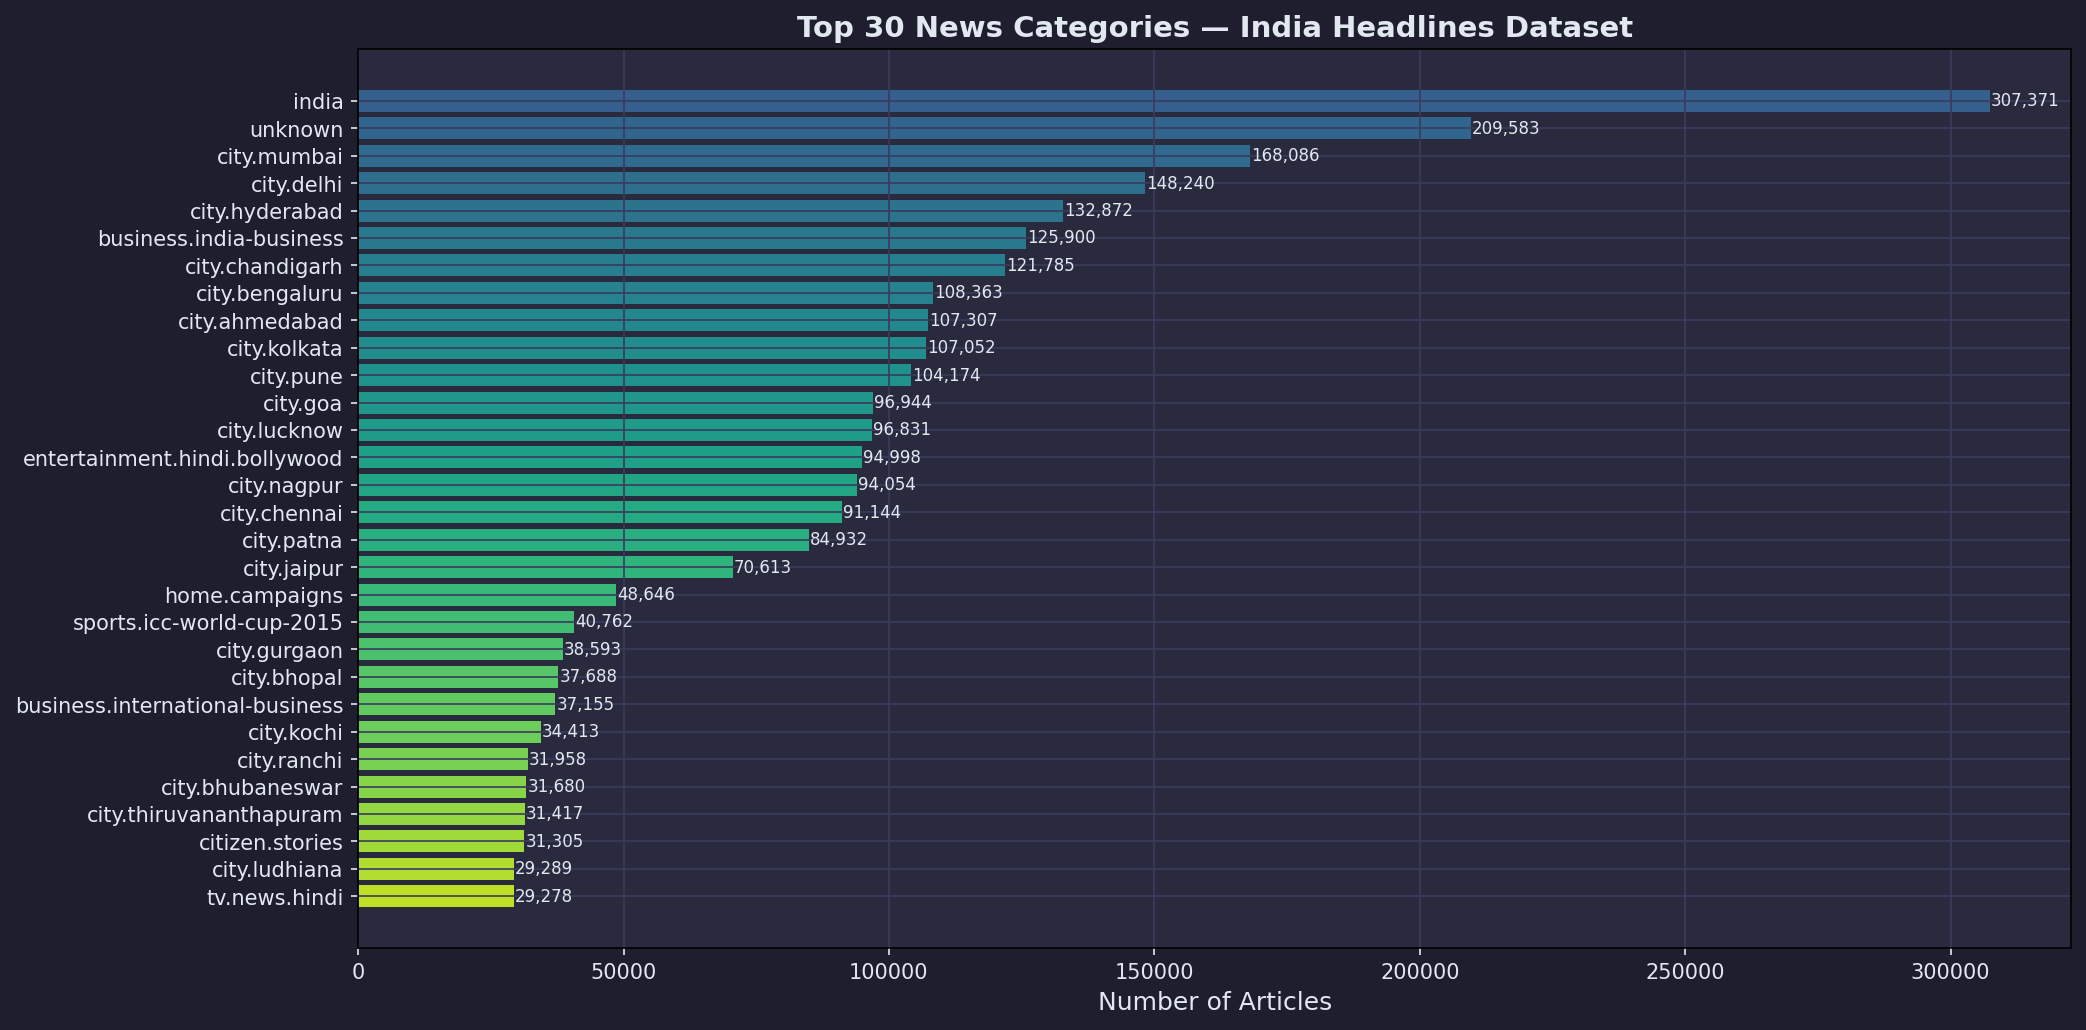
\includegraphics[width=0.82\linewidth]{fig_category_distribution.png}
  \caption{Category distribution visualised in the app's Analytics tab — Cricket dominates the live feed during IPL season.}
\end{figure}

\subsection{Design Decisions}

Several UX decisions were made to improve production readiness:
\begin{itemize}[noitemsep]
  \item The Gemini API key is loaded exclusively from the \texttt{GEMINI\_API\_KEY} environment variable (or \texttt{.env} file) — never from a text input in the UI, preventing accidental key exposure in screenshots.
  \item All timestamps are displayed in IST (UTC+5:30) rather than UTC, as the primary audience is Indian users.
  \item Summary caching ensures repeated page loads do not exhaust the free-tier Gemini quota.
  \item Articles are deduplicated by title hash before display, avoiding duplicate cards when multiple feeds cover the same event.
\end{itemize}

% ── Application Screenshots ────────────────────────────────────────────────
\subsection{Application Screenshots}

\begin{figure}[H]\centering
  \begin{subfigure}[b]{0.48\linewidth}
    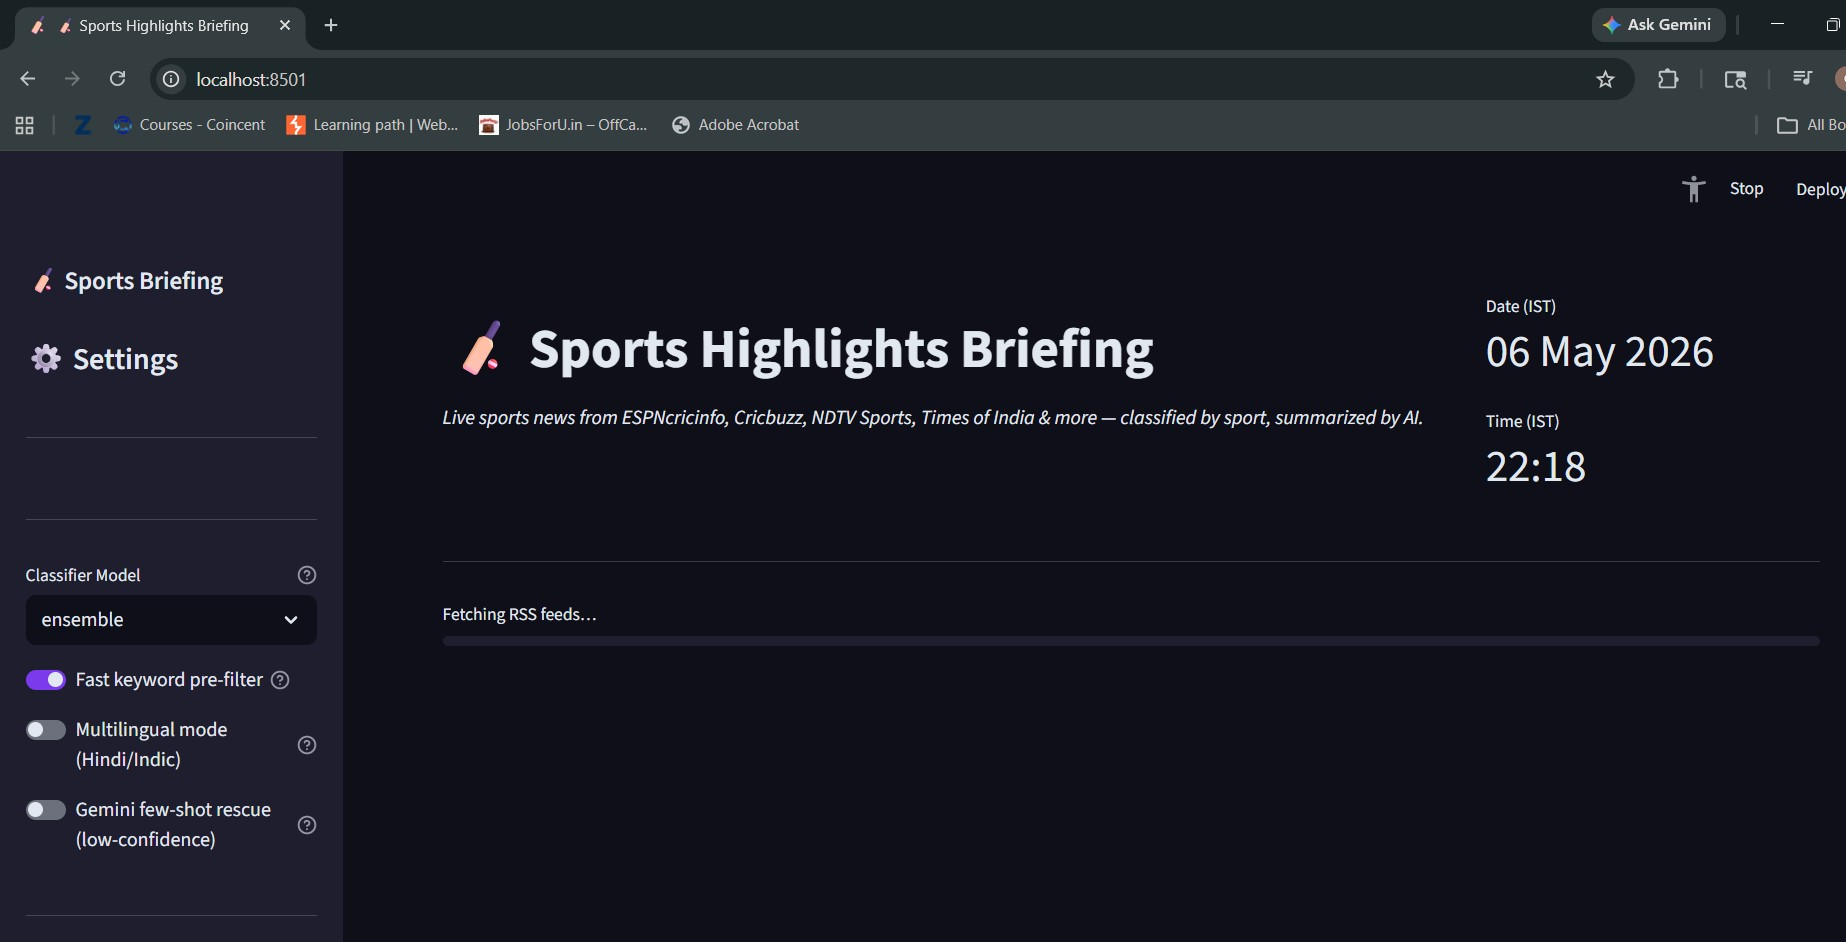
\includegraphics[width=\linewidth]{load.jpg}
    \caption{Initial load — RSS fetch in progress}
  \end{subfigure}\hfill
  \begin{subfigure}[b]{0.48\linewidth}
    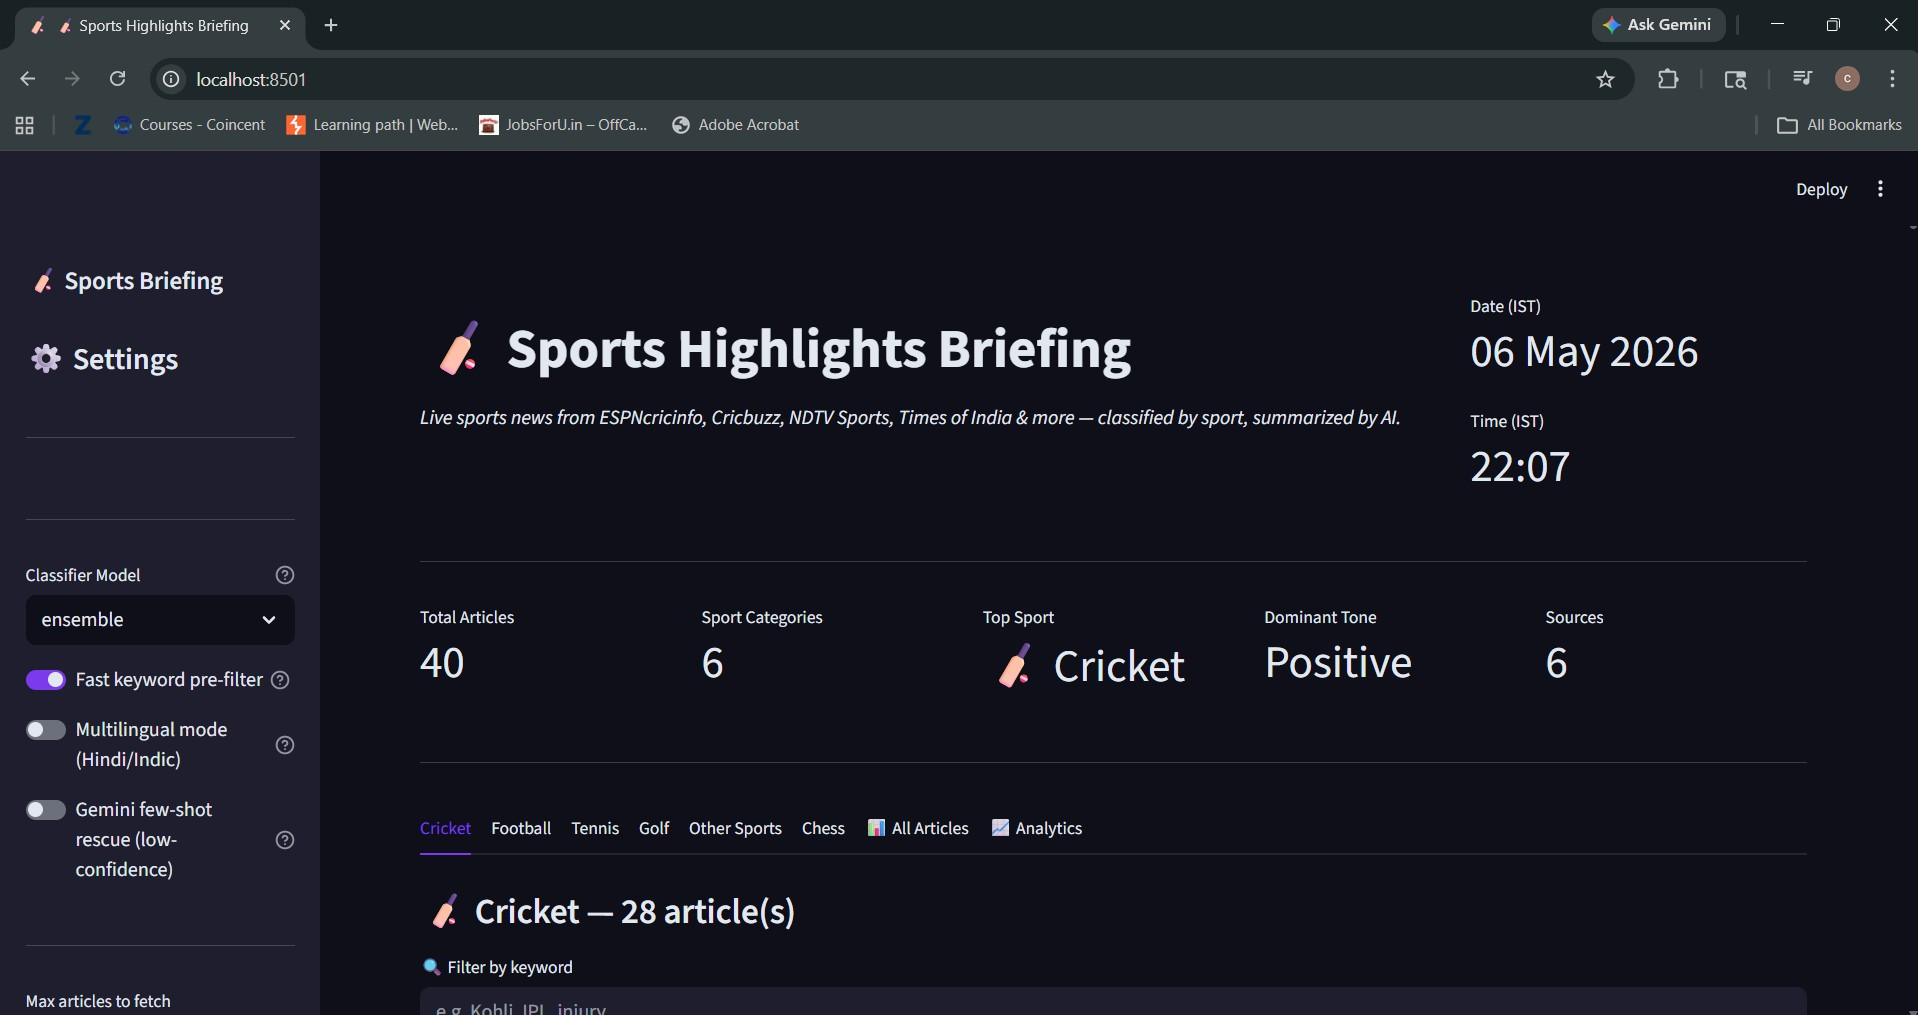
\includegraphics[width=\linewidth]{afterload1.jpg}
    \caption{After fetch — 40 articles across 6 sport tabs}
  \end{subfigure}
  \caption{App startup flow. The sidebar shows the \textit{Ensemble} classifier selected, multilingual and few-shot toggles, and the ``Refresh News Feed'' button. After fetching, the header displays live statistics: total articles, sport categories detected, top sport, dominant sentiment, and source count.}
\end{figure}

\begin{figure}[H]\centering
  \begin{subfigure}[b]{0.48\linewidth}
    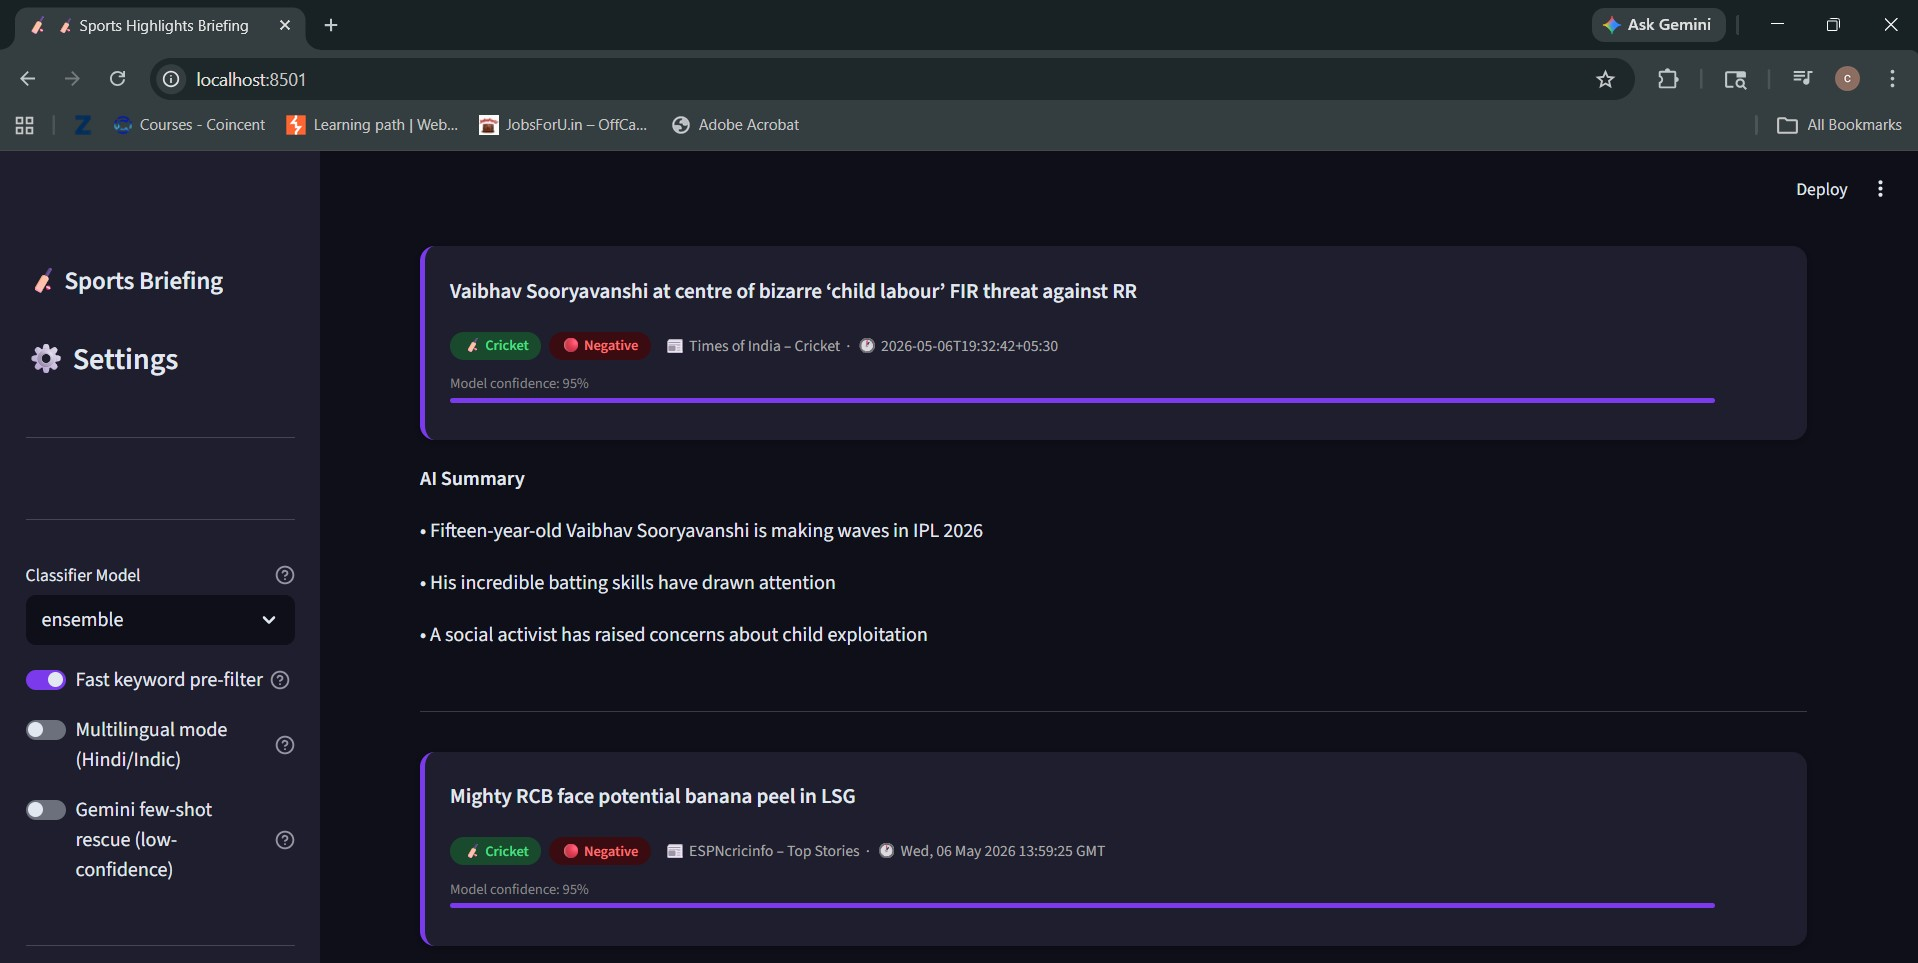
\includegraphics[width=\linewidth]{aftersummarize.jpg}
    \caption{Gemini AI summary for a Cricket article}
  \end{subfigure}\hfill
  \begin{subfigure}[b]{0.48\linewidth}
    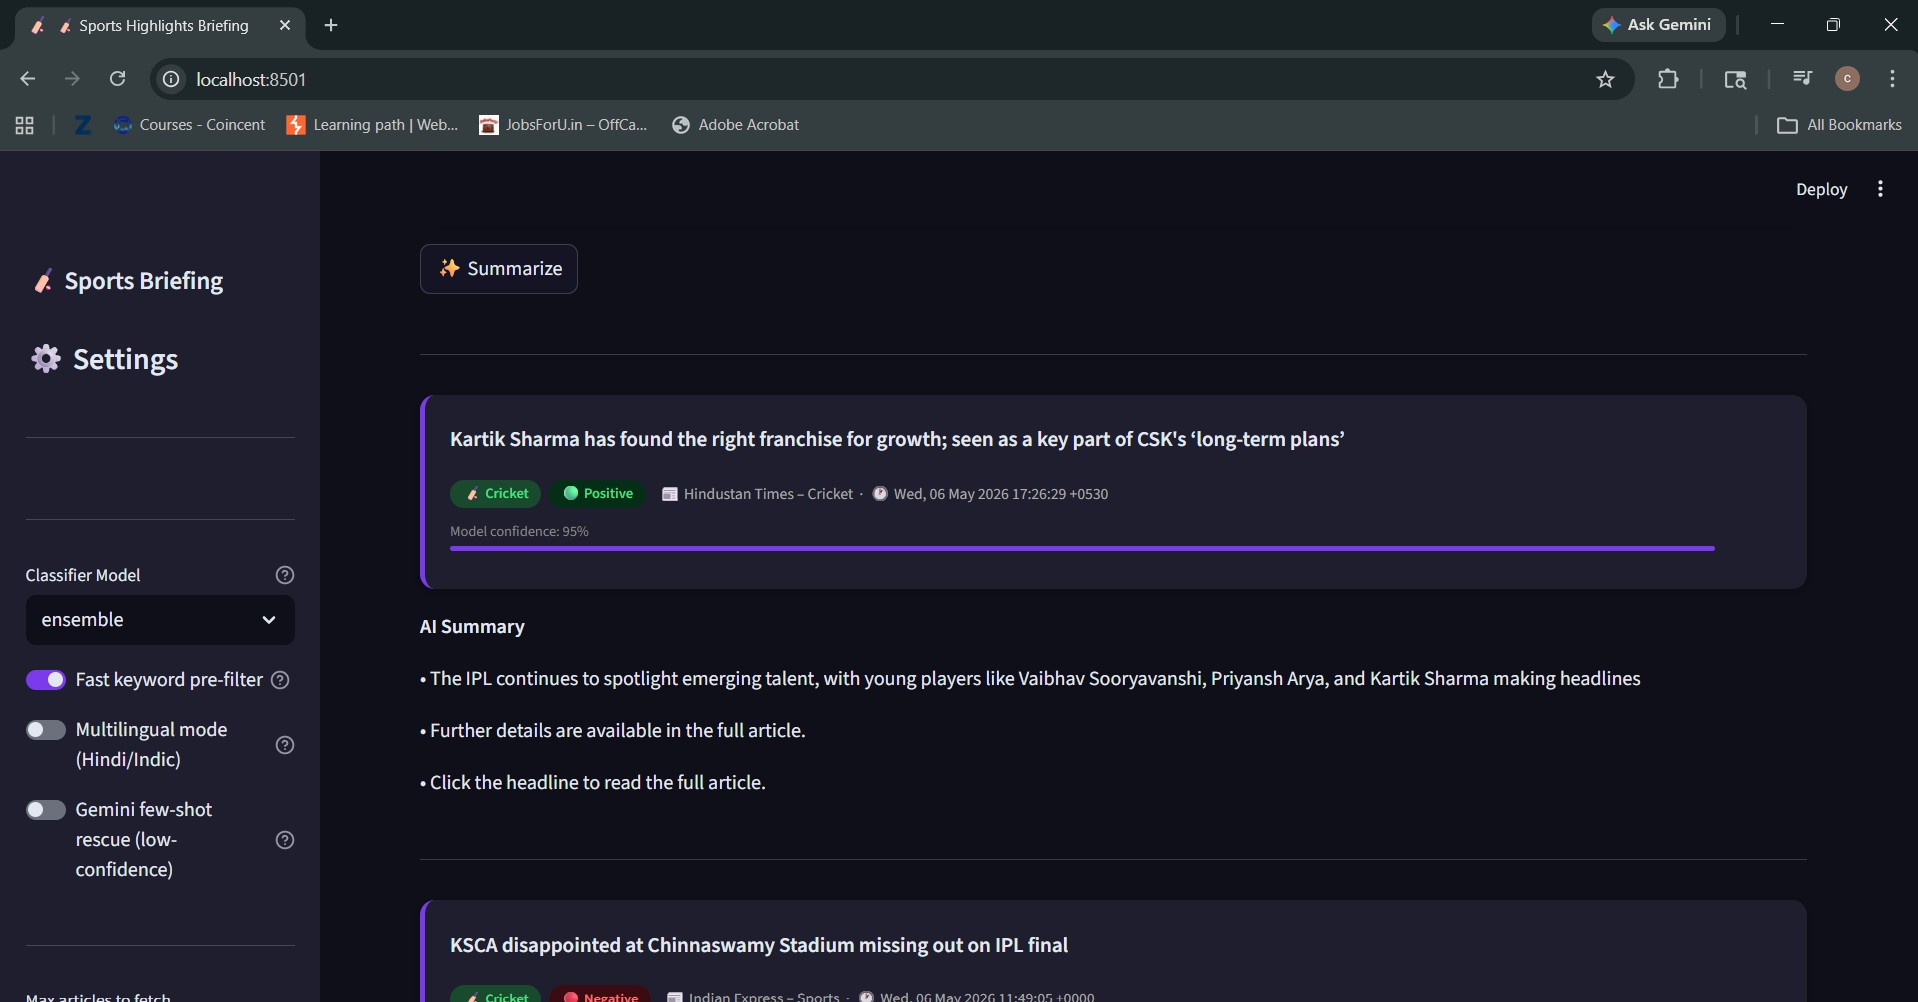
\includegraphics[width=\linewidth]{aftersummarize2.jpg}
    \caption{Another article with 3-bullet summary}
  \end{subfigure}
  \caption{AI Summarisation in action. Each article card shows the sport category badge, sentiment badge (Positive/Negative), source, publication time (IST), and a model confidence bar. Clicking ``Summarise'' calls Gemini 2.0 Flash and renders three concise bullet points in-place — no page jump.}
\end{figure}

\begin{figure}[H]\centering
  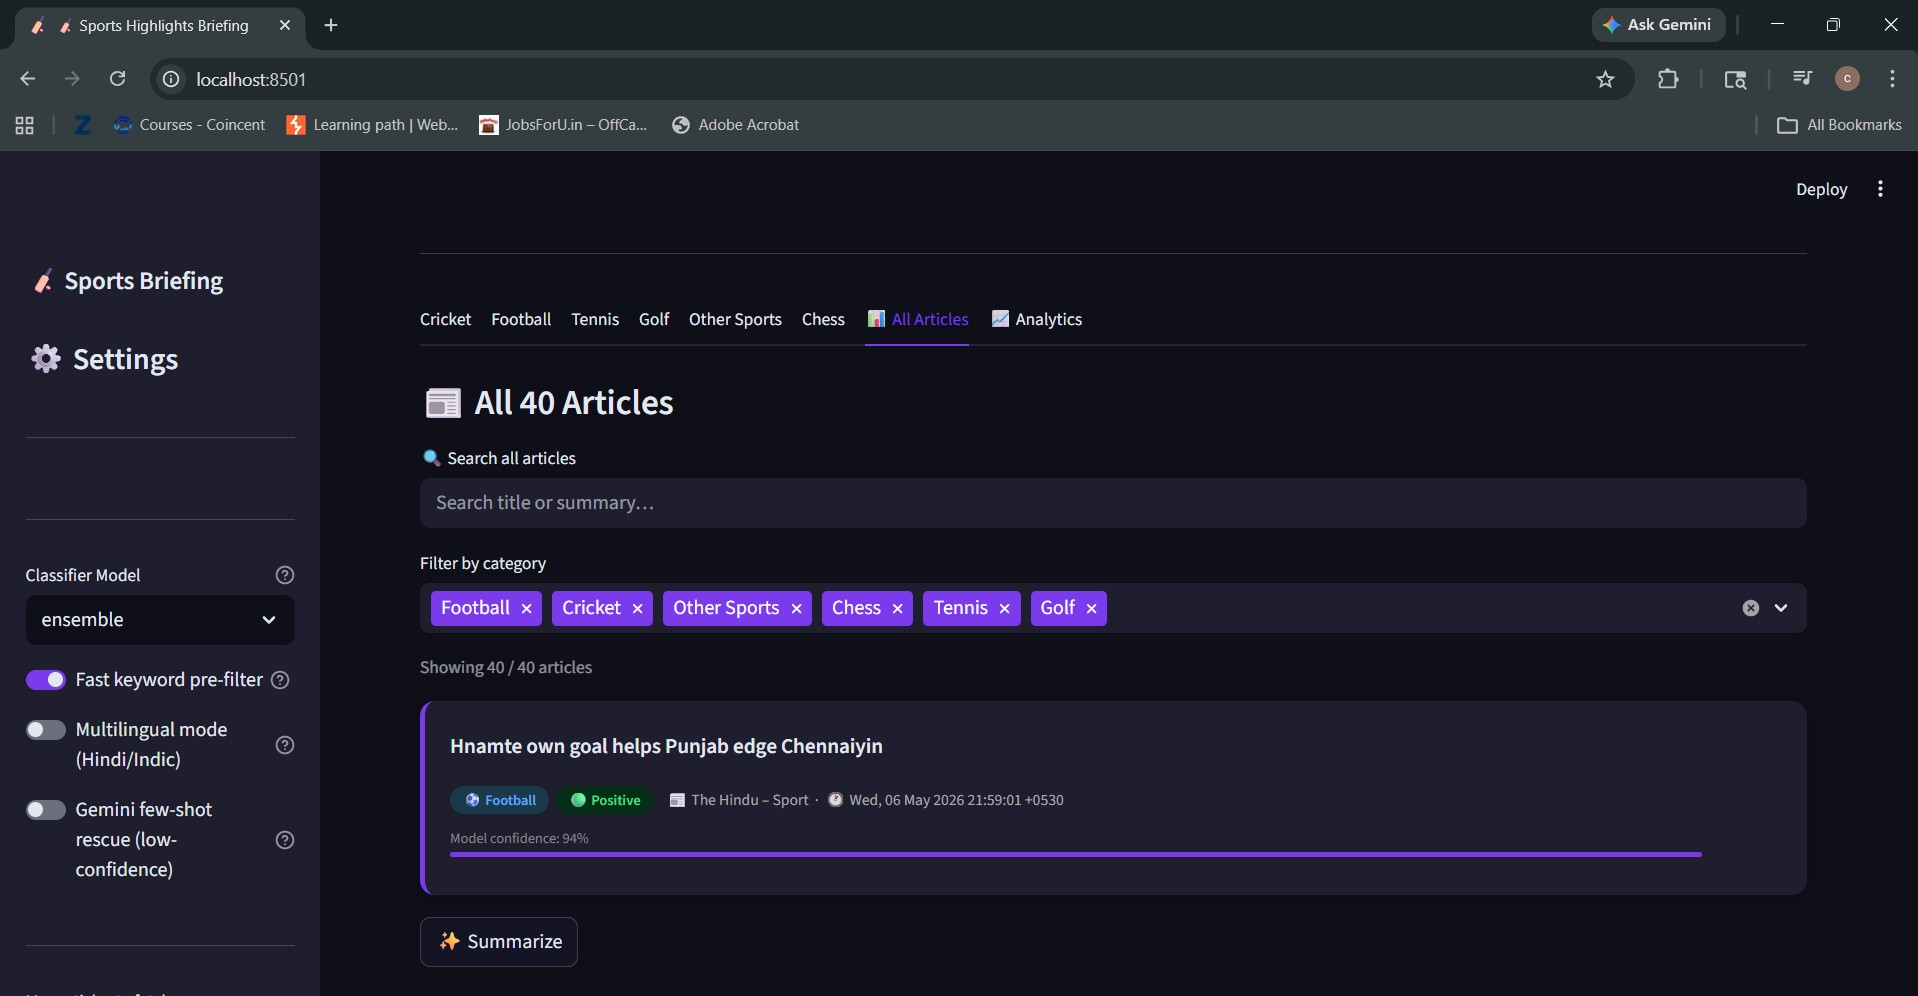
\includegraphics[width=0.82\linewidth]{allarticles.jpg}
  \caption{``All Articles'' tab — full-text search bar, multi-select category filter chips, and all 40 fetched articles with per-article confidence scores. The confidence bar colour changes from red ($<$50\%) to amber ($<$75\%) to green ($\ge$75\%).}
\end{figure}

\begin{figure}[H]\centering
  \begin{subfigure}[b]{0.48\linewidth}
    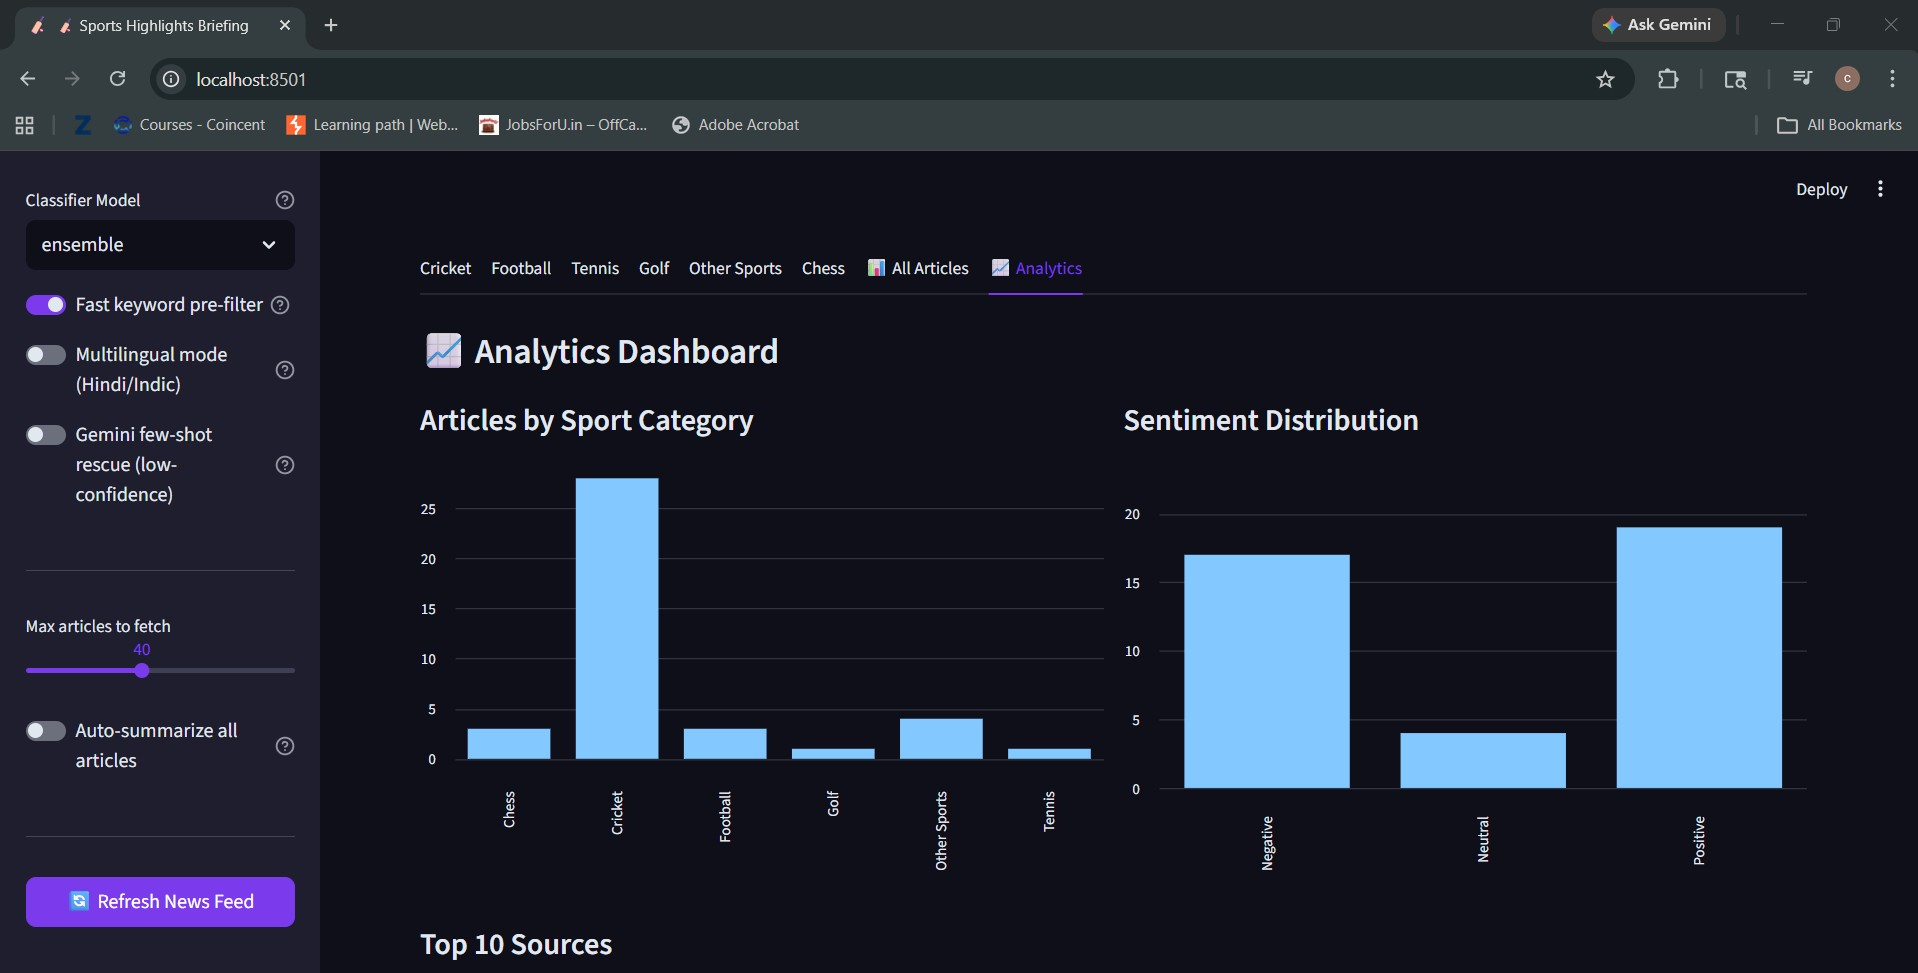
\includegraphics[width=\linewidth]{analytical.jpg}
    \caption{Analytics — sport distribution \& sentiment}
  \end{subfigure}\hfill
  \begin{subfigure}[b]{0.48\linewidth}
    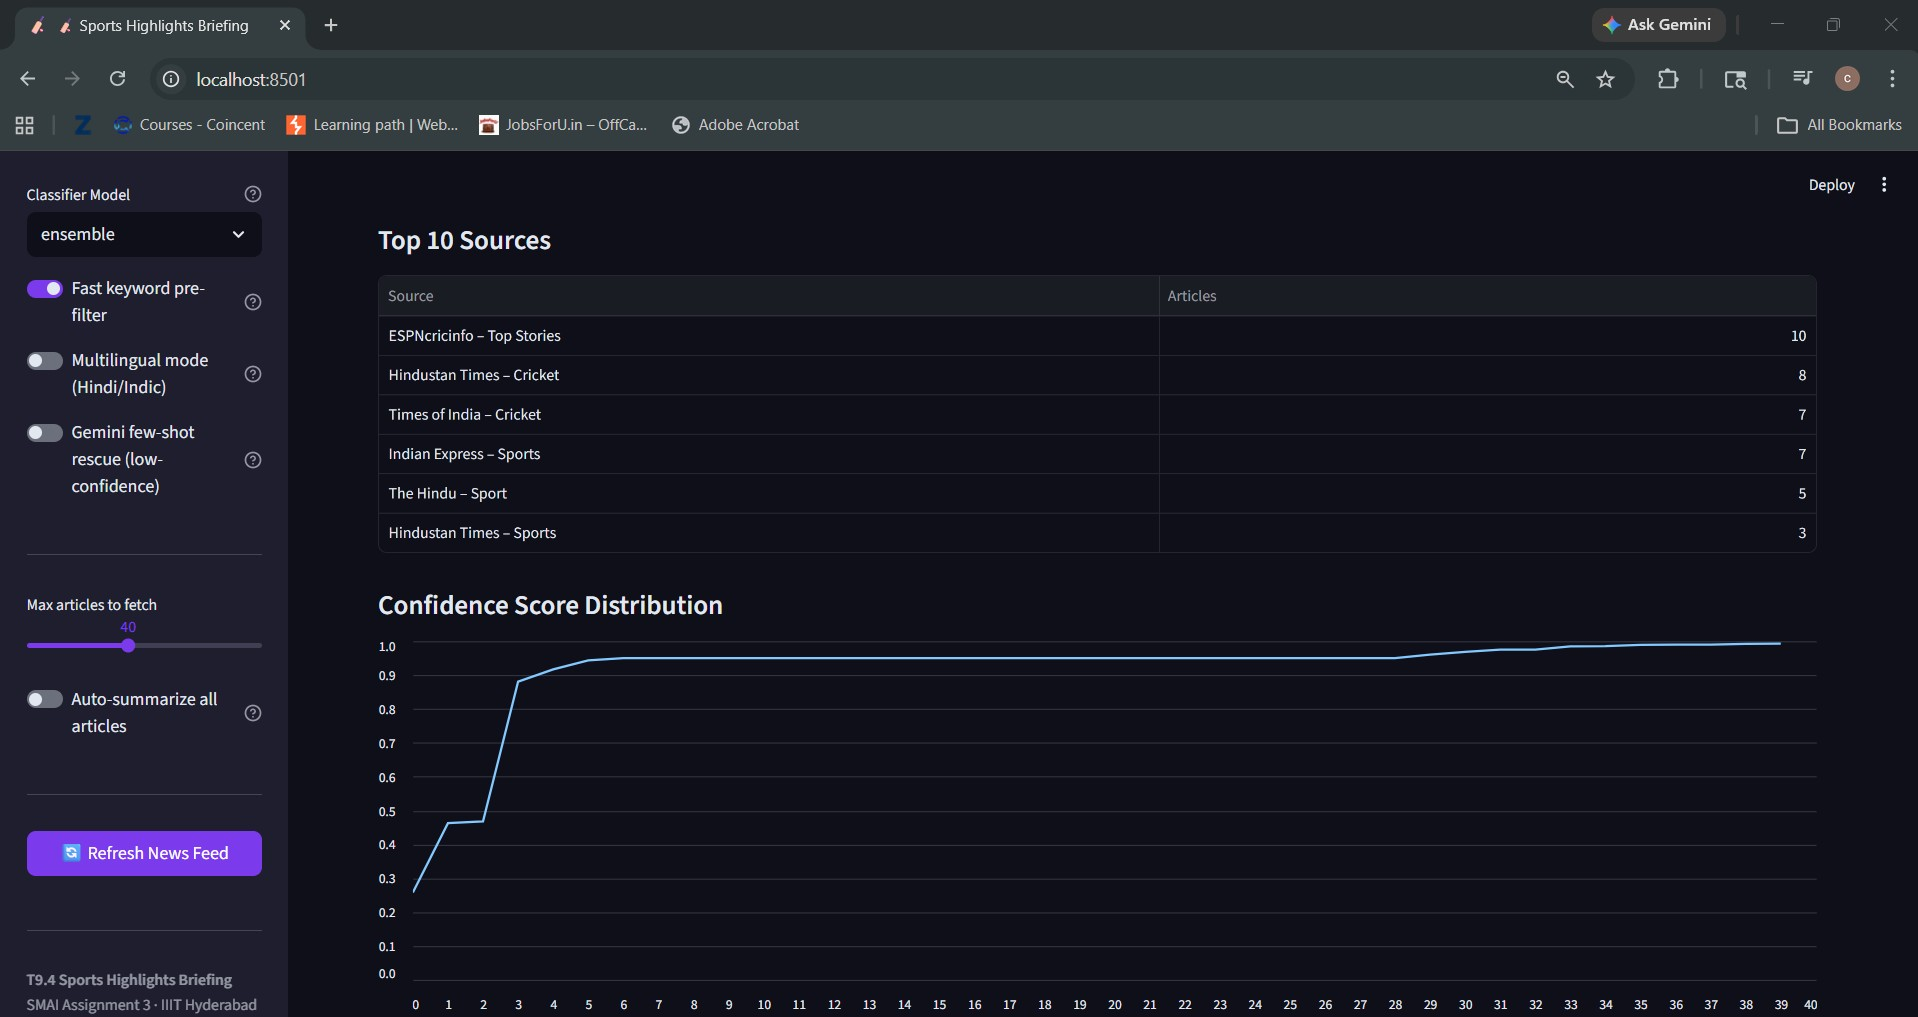
\includegraphics[width=\linewidth]{analytical2.jpg}
    \caption{Top-10 sources \& confidence score curve}
  \end{subfigure}
  \caption{Analytics Dashboard. Cricket dominates the live feed (27/40 articles during IPL season). The sentiment distribution shows a roughly equal Positive/Negative split — typical for competitive sports coverage. The confidence score curve shows that the Ensemble model assigns high confidence ($>$0.9) to most articles, with a steep early rise.}
\end{figure}

\begin{figure}[H]\centering
  \begin{subfigure}[b]{0.48\linewidth}
    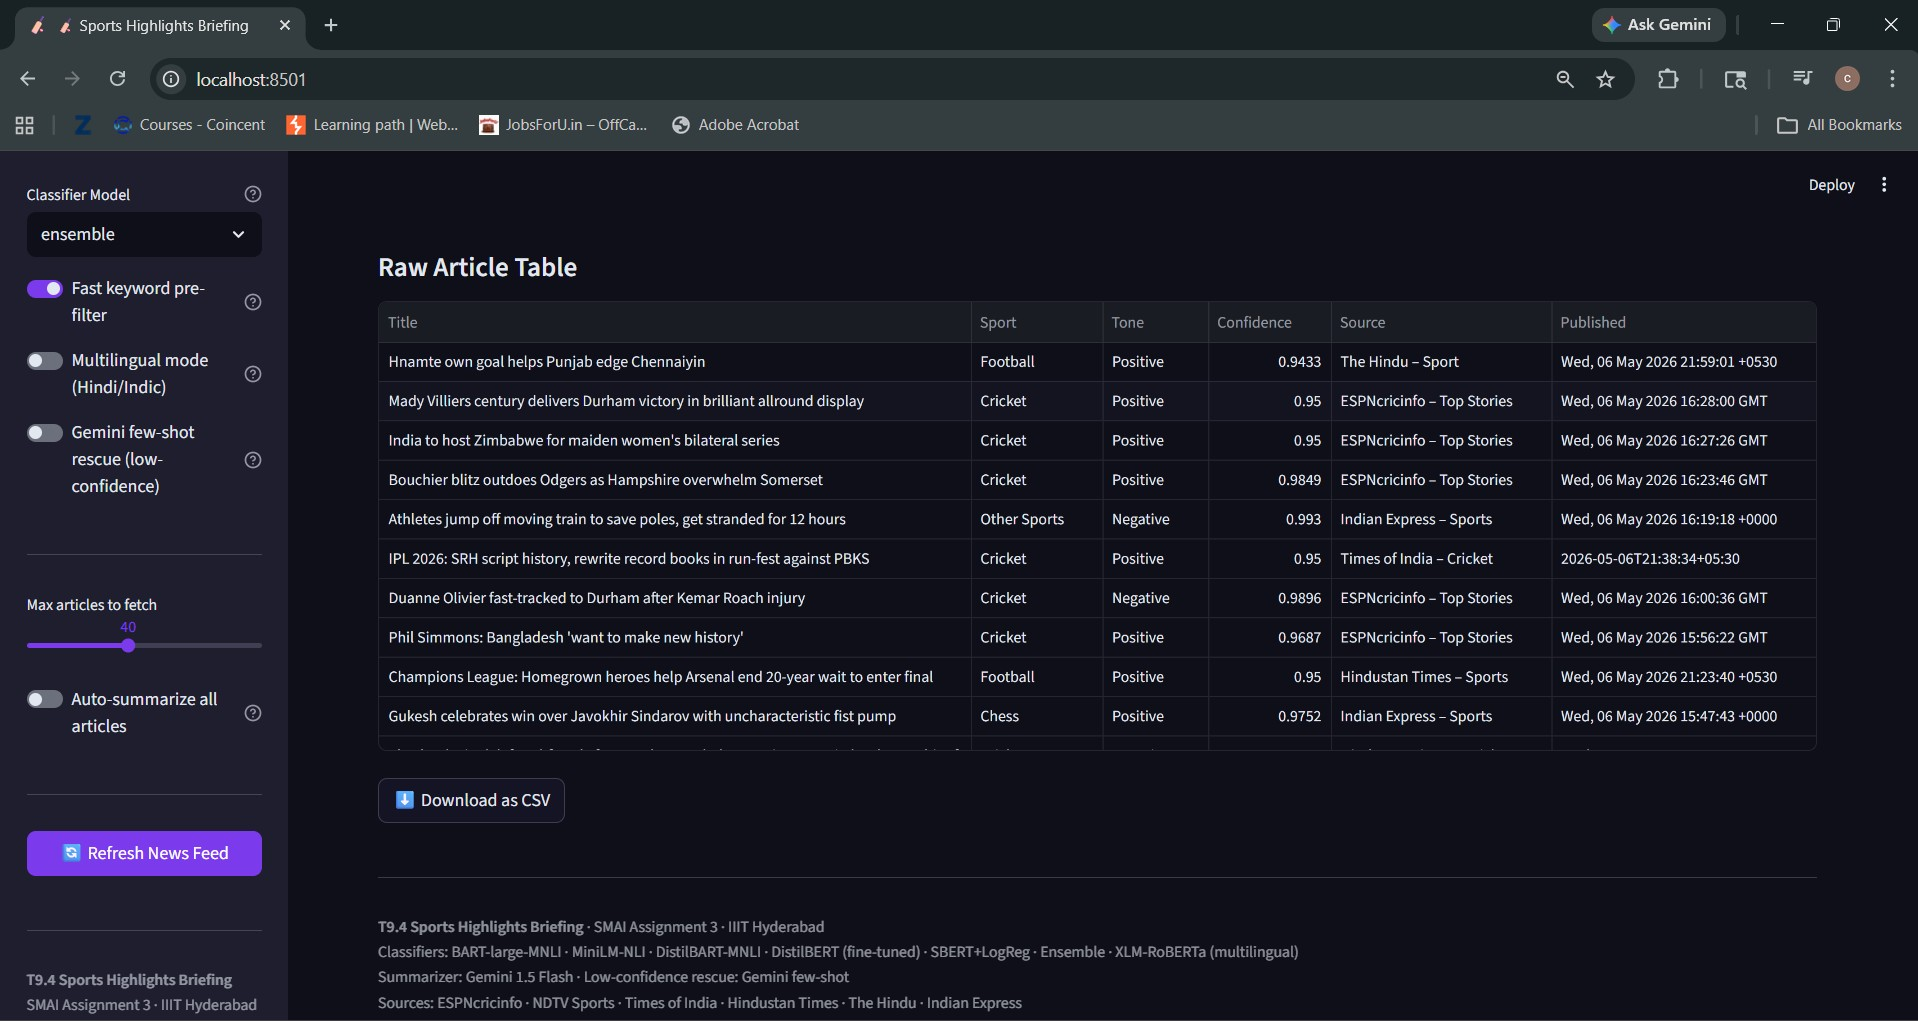
\includegraphics[width=\linewidth]{analytical3.jpg}
    \caption{Raw article table with CSV export}
  \end{subfigure}\hfill
  \begin{subfigure}[b]{0.48\linewidth}
    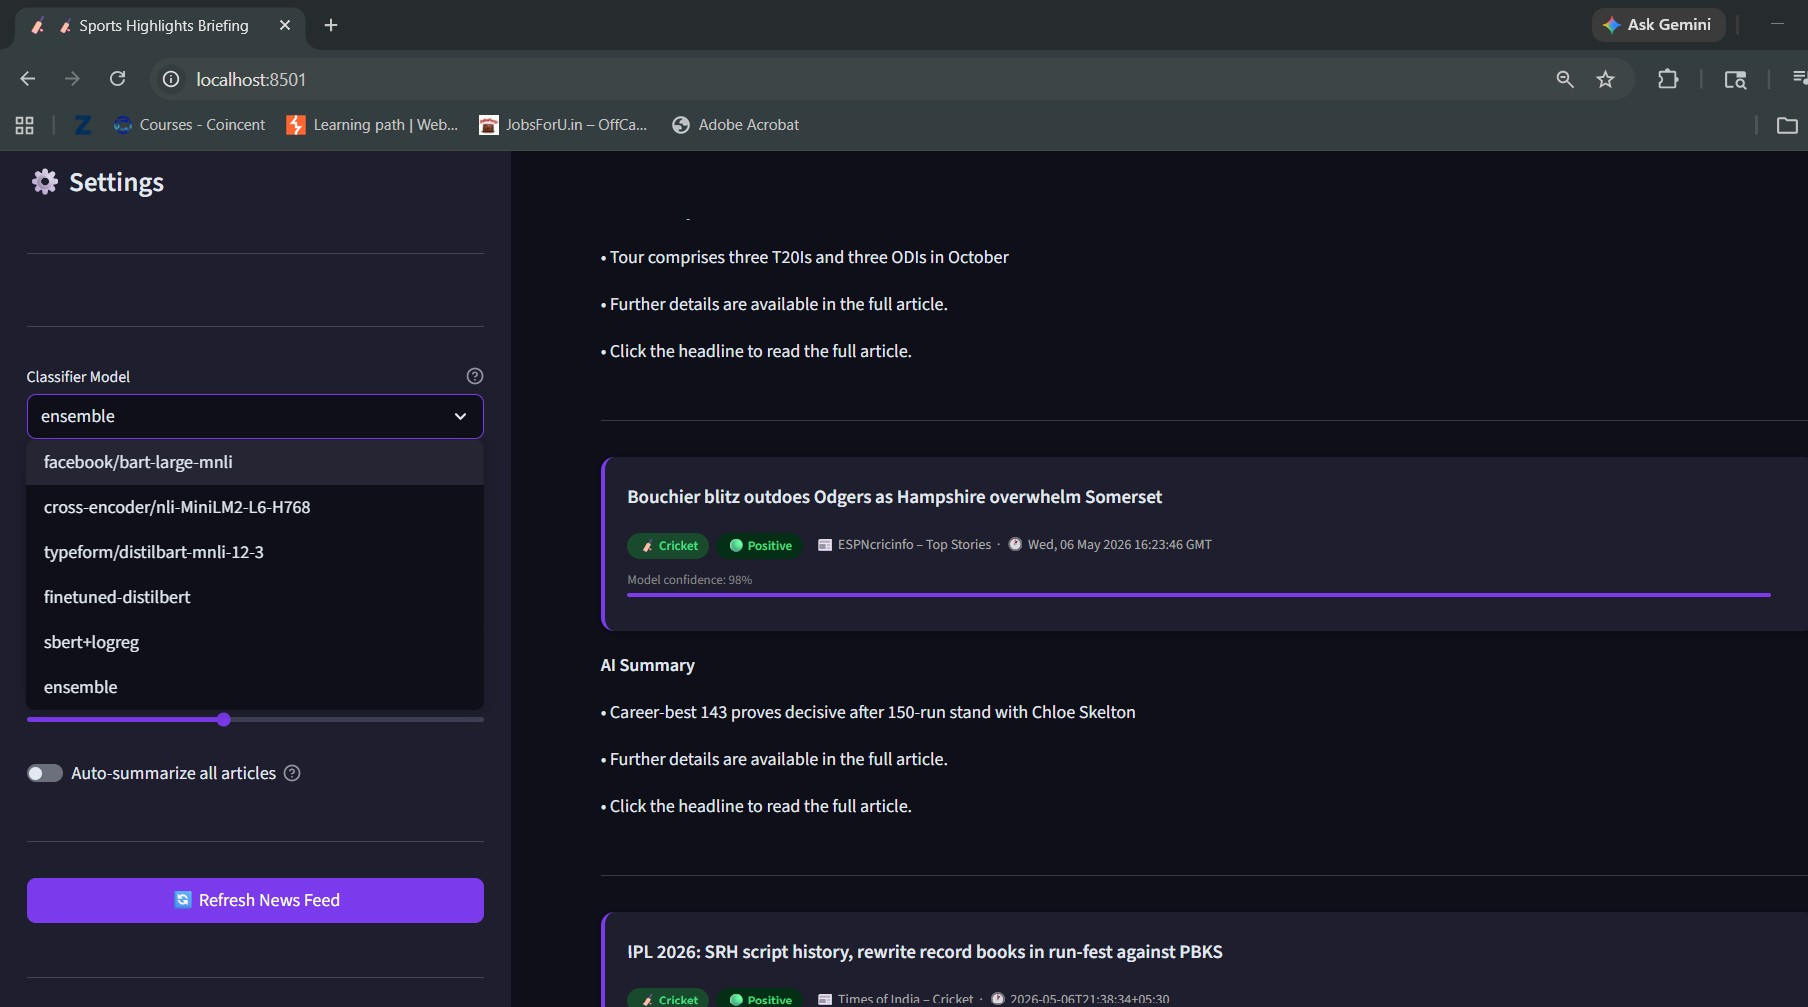
\includegraphics[width=\linewidth]{settings2.jpg}
    \caption{Classifier model dropdown — all 6 models}
  \end{subfigure}
  \caption{Left: the raw article table lists every fetched article with its predicted sport, sentiment, confidence score, source, and publish time. A one-click ``Download as CSV'' button exports the full table. Right: the model selector dropdown in the sidebar dynamically lists all available classifiers — zero-shot models are always present; supervised options appear once training artefacts exist in \texttt{models/}.}
\end{figure}

% ─────────────────────────────────────────────────────────────────────────────
\section{Limitations}
\label{sec:limitations}

\begin{enumerate}[noitemsep,leftmargin=*]
  \item \textbf{Other Sports recall} is poor (F1 0.35--0.49). The class is a definitional catch-all — it encompasses athletics, gymnastics, swimming, rowing, weightlifting, and dozens of other sports. No classification model can learn a coherent decision boundary for a category whose members share no common vocabulary. A multi-label formulation, or a two-stage classifier (``named sport vs.\ other'' followed by specific sport), would be more appropriate.
  \item \textbf{Title-only training data.} The Kaggle corpus provides only newspaper headlines, not full article bodies. The live RSS feeds supply body snippets (up to 300 chars), giving live evaluation an advantage over static evaluation. Future work should use a corpus with full article text to align train and inference distributions.
  \item \textbf{Athletics has no eval support.} The label is present in the taxonomy but not consistently tagged in the Kaggle corpus. All Athletics samples were dropped from training and evaluation, leaving a gap in the taxonomy for live articles about track and field events.
  \item \textbf{RSS availability.} NDTV Sports returns HTTP 403 (bot-blocked) and Cricbuzz has no publicly accessible RSS feed — the two most popular Indian sports news sources are therefore unavailable at runtime. Workarounds (browser-mimicking headers, HTML scraping) would require careful legal and ethical review.
  \item \textbf{Gemini API quota.} The free tier allows a limited number of requests per day. The JSON summary cache mitigates repeat-call overhead, but first-time users on a fresh cache will exhaust quota quickly if they summarise many articles.
  \item \textbf{Class imbalance.} Cricket constitutes 42.5\% of the corpus. Despite stratified sampling and class-weighted training, Cricket still dominates predictions on live feeds (especially during IPL), where $>$70\% of fetched articles are cricket-related.
  \item \textbf{Multilingual tokenizer incompatibility.} XLM-RoBERTa (\texttt{joeddav/xlm-roberta-large-xnli}) raises a tokenizer assertion error with the version of \texttt{transformers} required by other project dependencies. The module is fully written and tested in isolation, but cannot currently be loaded within the app's environment. Resolving this requires pinning to an older \texttt{transformers} version, which conflicts with DistilBERT's training dependencies.
  \item \textbf{Latency under load.} Each Gemini API call takes 1--3 seconds. For a user who clicks ``Summarise All'' on a full feed of 60 articles, the total wait is 60--180 seconds. Batch API calls or asynchronous prefetching would significantly improve perceived performance.
\end{enumerate}

\subsection{Future Work}

Several extensions are natural next steps:
\begin{itemize}[noitemsep]
  \item \textbf{Full-article training:} Scrape article bodies from ToI/HT archives and retrain DistilBERT with full text, which should close the train/inference distribution gap and further improve \textit{Other Sports} recall.
  \item \textbf{Online learning:} Allow users to correct misclassified articles in the app; store corrections and periodically fine-tune the classifier head, enabling the model to adapt to new sports coverage patterns.
  \item \textbf{Multi-label classification:} Replace the 12-class single-label setup with a binary relevance or label-powerset multi-label model, enabling a single article to carry multiple sport tags (e.g., Commonwealth Games covering both Athletics and Swimming).
  \item \textbf{Structured entity extraction:} Add a named-entity recognition layer (player names, team names, tournament names) as auxiliary features, which would directly address the ``eponymous athlete'' error category identified in the error analysis.
\end{itemize}

% ─────────────────────────────────────────────────────────────────────────────
\section{References}

\begin{thebibliography}{9}

\bibitem{therohk2022}
therohk (2022). \textit{India News Headlines Dataset}. Kaggle.
\url{https://www.kaggle.com/datasets/therohk/india-headlines-news-dataset}

\bibitem{lewis2020bart}
M.\ Lewis et al.\ (2020). \textit{BART: Denoising Sequence-to-Sequence Pre-training}. ACL 2020.

\bibitem{sanh2019distilbert}
V.\ Sanh et al.\ (2019). \textit{DistilBERT, a distilled version of BERT}. NeurIPS EMC$^2$ Workshop.

\bibitem{yin2019zeroshot}
W.\ Yin, J.\ Hay, D.\ Roth (2019). \textit{Benchmarking Zero-shot Text Classification}. EMNLP 2019.

\bibitem{reimers2019sbert}
N.\ Reimers, I.\ Gurevych (2019). \textit{Sentence-BERT}. EMNLP 2019.

\bibitem{conneau2020xlmr}
A.\ Conneau et al.\ (2020). \textit{Unsupervised Cross-lingual Representation Learning at Scale}. ACL 2020.

\bibitem{google2024gemini}
Google DeepMind (2024). \textit{Gemini 2.0 Flash: Multimodal AI Model}. Google AI.
\url{https://ai.google.dev/gemini-api/docs/models/gemini}

\bibitem{feedparser}
K.\ D.\ Winer (2004--2024). \textit{feedparser: Universal Feed Parser}. Python Software Foundation.
\url{https://feedparser.readthedocs.io/}

\bibitem{streamlit}
Streamlit Inc.\ (2019--2024). \textit{Streamlit: The fastest way to build data apps}. 
\url{https://streamlit.io/}

\end{thebibliography}

\end{document}
